\documentclass[12pt]{article}
\usepackage{geometry}
\geometry{a4paper, total={170mm,257mm},left=20mm, top=20mm,}
\usepackage[colorlinks=true,linkcolor=blue,urlcolor=black]{hyperref}
\usepackage{bookmark}
\usepackage{graphicx}
\usepackage[autostyle, english = american]{csquotes}
\usepackage{appendix}
\usepackage{float}
\begin{document}
\begin{titlepage}
\centering
\vfill
\vspace*{4\baselineskip}
{\bfseries\Large
Labtainer Lab Designer User Guide\par
}
\vspace*{4\baselineskip}
{\bfseries
Fully provisioned cybersecurity labs\par
}
\vspace*{2\baselineskip}
\today
\vfill
%
\includegraphics[natwidth=200, natheight=286]{labtainer5-sm.png}

\includegraphics[width=0.4\textwidth]{labtainer5-sm.png}
\vfill

\vspace{2.0in}
This document was created by United States Government employees at 
The Center for Cybersecurity and Cyber Operations (C3O) at the Naval Postgraduate School NPS. 
Please note that within the United States, copyright protection is not available for any works created  
by United States Government employees, pursuant to Title 17 United States Code Section 105.   
This document is in the public domain and is not subject to copyright. 
\end{titlepage}
\tableofcontents
\newpage
\section {Introduction}
This manual is intended for use by lab designers wanting
to create or adapt cybersecurity labs to use the Docker
container-based lab framework known as ``Labtainers''.
The Labtainer framework is designed for use with computer and network security
laboratory exercises targeting Linux environments, and it is built around 
standard Linux Docker containers.  A Labtainer exerciese may include multiple 
networked components, all running locally on a student's computer, but without
the performance degredation associated with running multiple virtual machines.

While most Labtainer exercises focus on exploring concepts via the Linux command line -- GUI based
applications, e.g., browsers and Wireshark are also supported. 

\subsection {Benefits of Labtainers}

Deploying cybersecurity labs using this framework
provides three primary benefits:

\begin{enumerate}
\item The lab execution environment is controlled and consistent
across all student computers regardless of the Linux distribution
and configuration present on individual student computers.  
This allows each lab designer to control
which software packages are present, the versions of libraries and
specific configuration settings, e.g., /etc file values. These configurations
may vary between labs, and they may vary between multiple computers in
a single lab.

\item Assessment of student lab activity can be automated through a
set of configuration files that identify expected results, thus
relieving lab instructors from having to individually review detailed lab
results.

\item Labs may be automatically ``parameterized'' for each student such that
students cannot easily copy results from another student or from internet
repositories.  
\end{enumerate}

Labtainers provide the advantages of a consistent
execution environment without requiring
an individual Virtual Machine (VM) per lab, and without requiring all labs to be adapted for
a common Linux execution environment.   These benefits can be realized 
whether or not labs are configured for automatic assessment, 
or are parameterized for each student.

\begin{figure}[H]
\centering
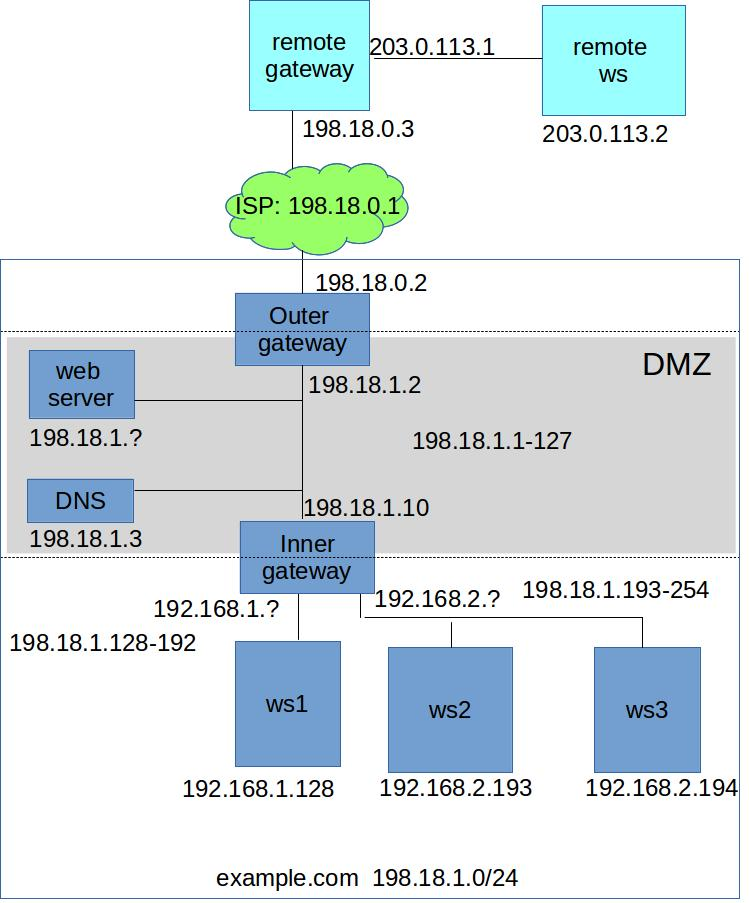
\includegraphics[width=0.4\textwidth]{dmz-lab.jpg}
\caption{Example Labtainers network topology}
\label{fig:dmz}
\end{figure}

Exercises that include multiple networked computers illustrate an advantage 
of using containers over VMs, namely, containers require significantly less resources
than do VMs.  A student laptop that struggles to run two or more VMs can readily 
run multiple containers simultaneously, as shown in this 50 second demonstration: \url{https://youtu.be/JDV6jGF3Szw} 

Lab designers enhance labs to include automated assessment using directives built into the famework.
For example, ten rather simple directives can evaluate the following question regarding a student'
work on a lab depicted in Figure \ref{fig:dmz}:

``Was there any
single iptables configuration during which the student used nmap to demonstrate that:
\begin{itemize}
\item The remote workstation could reach the HTTPS port but not the SQL port, and,
\item The local workstation could reach the HTTPS port and the SQL port.''
\end{itemize}

\subsection {Obtaining the Labtainer development kit}
Installation of Labtainers is described in the \textit{Labtainer Student Guide},  
which also includes instructions for installing an Ubuntu VM (if you do not already have a Linux system),
and the Labtainer framework.  Our website also distributes pre-packaged VM appliances that already have
Labtainers installed. Labtainers will work with any Linux
distribution that supports Docker containers.  If you already have Docker installed on a Linux system, 
reference the Student Guide for other dependencies. 

The difference between the development kit and the standard Labtainer distribution is primarily
just the lab definition files, which are withheld from the general distribution for efficiency.


If you have a Labtainer installation (e.g., our pre-packaged VM), you can get the developer files by going to your
labtainers directory, e.g., {\tt \~{}/labtainer/} and running {\tt ./update-designer.sh}
\footnote{The student password for the pre-packaged VM is "password123".}
You may then want to logout and login again, or run a new {\tt bash} shell because that script
sets some environment variables.

It is suggested that you periodically run that update script to get the latest lab definition files,
and to update framework software.   

\subsection{Content of this guide}
This guide describes how to build new labs, but first, section \ref{student environment}
gives an overview of how students interact with Labtainers.  The steps taken to
create a new lab are provided in section \ref{sec:new_labs}, and the mechanics of defining
the lab execution environment are in section \ref{execution environment}.

Individualizing labs to discourage sharing of solutions is described in \ref{parameterize}.
Section \ref{assessment} then describes how to define criteria to enable automated assessment
of student work.  

Networking considerations are described in \ref{networking}.  Section \ref{publishing} covers
the process of building, publishing and maintaining labs.

Strategies for creating mulit-user Labtainer exercises are discussed in section \ref{multi user}.
Section \ref{limitations} identifies limitations of the framework and section \ref{Notes} includes
application-specific notes, e.g., notes relavent to including Firefox in a lab.

Automated testing of labs is supported using our SimLab tool as described in Appendix \ref{testing}.


\section {Overview of the student environment and workflow}
\label{student environment}
Labtainers support laboratory exercises designed for Linux environments,
ranging from interaction with individual programs to labs that include
what appear to be multiple components and networks.  Students see and interact with Linux
computers, primarily via bash shell commands and GUI-based applications. In general, the Labtainer
framework implementation is not visible to the student, and the Linux
environment as seen by the student is not noticeably augmented to support the framework.

Labtainers are intended for use on individual student computers, e.g., a laptop,
or potentially a VM allocated to the student from within a VM farm. \footnote{Labtainers
can also support labs in which students collaborate (or compete) on shared infrastructure.
Please see section \ref{multi user} for information on multi-user environments.}
The computer utilized by a student must include the Linux operating system, e.g.,
as a single VM.  This Linux operating system, referred to herein
as the \textit{Linux host}, can be any distribution and version
which supports Docker.  Students download and expand a tarball, and run
an installation script as described in the \textit{Labtainer Student Guide}
\footnote{This tarball may someday be replaced by standard Linux distribution packages,
e.g., Debian and/or RPM packages.} Alternately, students can use a Linux VM
that is pre-configured with Labtainers and Docker, and is available at our website.

It is suggested that the student's Linux host be a virtual machine that is
not used for purposes requiring trust.  Software programs contained in cybersecurity lab
exercises are not, in general, trusted.  And while Docker containers provide namespace
isolation between the containers and the Linux host, the containers run as privileged.

Labtainer exercises can include networking to external hosts, e.g., a Windows VM
running alongside the Linux host VM, as described in section \ref{external hosts}.

Students initiate any and all labs from a
single workspace directory on the Linux host.
To perform a specific Labtainer exercise, the student runs a \textit{labtainer} command from
the Labtainer workspace, naming the lab exercise.  This results in one or more
containers starting up along with corresponding virtual terminals via which the 
student will interact with the containers.  These virtual terminals typically
present a bash shell.  Each container appears to the student as a separate
computer, and these computers may appear to be connected via one or more networks.  

When a student starts a given exercise for the first time, the framework fetches
Docker images from the Docker registry.  Docker manages container images as a set of
layers, providing efficient storage and retrieval of images having common components.
The initial Labtainer installation step pulls a few baseline images (about 1.5 GB) from 
the public
Docker registry, known as the \textit{Docker hub}.  Images for specific labs are pulled
from the Docker hub by downloading only those additional layers required by that lab, and
which had not been previously pulled from the hub.  This is transparent to
the student, other than waiting for downloads to complete.

After the student performs the lab exercise, artifacts from the container
environments are automatically collected into an archive, (a zip file), that appears on
the student's Linux host.  The student forwards this archive file to the instructor,
e.g., via email or a learning management system (LMS).  The instructor collects student archive files into a common
directory on his or her own Linux host, and then issues a command that
results in automated assessment of student lab
activity, (if the lab is designed for that), and the optional creation of an environment
in which the instructor can review the work of each student.

Many cybersecurity lab exercises are assessed through use of reports in which students
describe their activities and answer specific questions posed by the instructor.  Labtainers
are intended to augment, rather than supplant this type of reporting.  The framework includes
mechanisms for automating the collection of student lab reports into the artifact archive files
that are collected by instructors. 


\section {Creating new labs}
\label{sec:new_labs}
The most challenging and critical part of designing a new cybersecurity lab
is the design of the lab itself, i.e., identifying learning objectives and
organizing exercises to achieve those objectives.  The Labtainer framework
does not specifically address any of that.  Rather, the framework is intended
to allow you to focus more time on the design of the lab and less time on mitigating and
explaining system administration and provisioning burdens you would otherwise place on 
students and instructors.

Typical steps for developing a new lab are:
\begin{enumerate}
\item Give the lab a name and create its computers using the {\tt new\_lab\_setup.py} script;
\item Choose the starting baseline configuration for each computer and add software packages
within a Dockerfile;
\item Define networks and connections to the lab computers in the lab's {\tt start.config} file.
\item Populate the user's HOME directory and system directories with lab-specific files.
\end{enumerate}
The remainder of this section covers the fist step and provides an example.  The 
following section \ref{execution environment}, covers the other three
steps.  After a lab is created, you can then optionally parameterize it per section \ref{parameterize} and/or
define criteria for automated assessment per section \ref{assessment}

\subsection{Create the first lab computer}
Labtainer exercises each have their own
directory under the ``labs'' directory in the project repository.
The first step in creating a new lab within the framework is to create
a directory for the lab and then cd to it.  The directory name will be the name
used by students when starting the lab.  It must be all lower case and not contain spaces.
\begin{verbatim}
    cd $LABTAINER_DIR/labs
    mkdir <new lab name>
    cd <new lab name>
\end{verbatim}

\noindent After the new lab directory is created, run the ``new\_lab\_setup.sh'' script.
\footnote {The {\tt \$LABTAINER\_DIR} will have been defined in your .bashrc
file when you installed Labtainers.  It should point to the {\tt labtainers/trunk}
directory.  You may need to start a new {\tt bash} shell to inherit the environment
variable.}

\begin{verbatim}
    new_lab_setup.py
\end{verbatim}
This will create a set of template files that you can then customize
for the new lab.  These template files are referenced in the discussion
below.
The result of running {\tt new\_lab\_setup.py} is a new labtainer lab that can be immediately run.  
While this new lab will initially only present you with a bash shell to an
empty directory on a Linux computer, it is worth testing the lab to understand the workflow.

\subsection{Testing the new lab}
Once a new lab directory is created, and the new\_lab\_setup.py has been run, then 
you can test the new, (currently empty) lab.  All student labs are launched from the
labtainer-student directory.  Lab development workflow is easiest if at least two
terminals or tabs are used, one in the new lab directory, and one in the labtainer-student
directory.  So, open a new tab or window, and then:

\begin{verbatim}
    cd $LABTAINER_DIR/scripts/labtainer-student
\end{verbatim}
Then start the lab using the:

\begin{verbatim}
    rebuild [labname] 
\end{verbatim}
command, where labname is the name of the lab you just created.  

The {\tt rebuild} command \footnote{Previously named {\tt rebuild.py}} will remove and recreate the lab containers
each time the script is run.  And it will rebuild the container images if any of their configuration 
information has changed.  \footnote{The build process may generate warnings in red text, some of which are expected.  
These include an unreferenced ``user'' variable and the lack of apt-utils if apt-get is used to install packages in 
Dockerfiles.}  This is often necessary when building and testing new labs, to ensure the
new environment does not contain artifacts from previous runs.
The progress of the build, and error messages can be viewed in 
the labtainer.log file.  While developing, it is generally a good idea to tail this log in
a separate terminal:
\begin{verbatim}
    tail -f labtainer.log
\end{verbatim}
If the rebuild fails with a error reflecting a problem resolving hostnames, e.g., mirror.centos.com, please see \ref{DNS-rebuild}.

Note the {\tt rebuild} command is not intended for use by students, they would use the ``labtainer'' command.  
The rebuild utility compares file modification dates to Docker image creation dates to determine if
a given image needs to be rebuilt.  The rebuild may miss file deletions.  Thus, if files are deleted, you must
force the rebuild using the {\tt -f} option at the end of the rebuild command. Also, addition of symbolic links will not
trigger a rebuild.  Rebuild references git modify dates (vice file modify dates).

Stop the lab with 
\begin{verbatim}
    stoplab
\end{verbatim}
When you stop the lab, a path to saved results is displayed.
This is the zip file that the student will forward to the instructor.

To test adding a ``hello world'' program to the new labtainer, perform the following steps:
\begin{itemize}
\item From the new lab directory window, cd \verb!$LABTAINER_DIR/labs/[labname]/[labname]!
\item Create a ``hello world'' program, e.g., in python or compiled C.
\item From the labtainer-student window, run {\tt rebuild [labname]}
\end{itemize}
    
You should see the new program in the container's
home directory.  If you run the program from the container, and then stop the lab
with stoplab, you will see the stdin and stdout results of the program within the
saved zip file.

The ``hello world'' program was placed in \verb!$LABTAINER_DIR/labs/[labname]/[labname]!.
The seemingly redundant ``labname'' directories are a naming convention in which the
second directory names one of potentially many containers.  In this simple example,
the lab has but one container, whose name defaults to the lab name.

The following sections describe how to further alter the lab execution environment seen by 
the student.

\subsection {Multiple containers}
The {\tt new\_lab\_setup.sh} script can be used to create additional containers for use
in the lab.  For example, from your new lab directory:
\begin{verbatim}
    new_lab_setup.py -a joe_computer
\end{verbatim}
\noindent will create a second container for your lab,
named ``joe\_computer''.  If you again run the rebuild script, you will see two virtual
terminals, each connected to one of your two independent computers.  Use 
\begin{verbatim}
    new_lab_setup.py -h
\end{verbatim}
\noindent to view the operations available in that script.

The following sections describe how to configure the execution environments on your components,
and how to define virtual networks connected to the components.

\section {Defining the lab execution environment}
\label{execution environment}
A given lab typically requires some set of software packages, and some
system configuration, e.g., network settings, and perhaps some lab-specific
files.  It can include multiple containers, each appearing as distinct
computers connected via networks.  The execution environment seen by a
student when interacting with one of these ``computers'' is therefore defined
by the configuration of the associated container. 

Software packages are defined in each container's Dockerfile, described in 
the subsection below. That is followed by subsection \ref{start config} describing network definitions,
(and other computer attributes) in the start.config file.  The remaining subsections then
described populating the user HOME directory and system directories, and methods for starting 
system services and miscellaneous environment settings. 

Labtainer containers, by default, present students with a virtual terminal and a bash
shell requiring no login.  Alternate initial environments, including use of the login program, are
described in section \ref{student start}.

Section \ref{persistent} describes how to
allow students to share tools they've developed between different labs.  

\subsection {Docker files}
A default Labtainer-specific Dockerfile is placed in the new lab's ``Dockerfiles'' 
directory when the new lab is created.  And additional Dockerfiles are added when the
{\tt new\_lab\_setup.sh -a} script adds computers to the lab. We use standard Docker file syntax, which is described at 
\url{https://docs.docker.com/engine/reference/builder/}

Simple labs should be able to use the default Dockerfile copied by the 
new\_lab\_setup.py script.  That Dockerfile refers to a base Labtainer
image that contains the minimum set of Linux packages necessary to 
host a lab within the framework.  The default
execution environment builds off of a recent Ubuntu image.

\noindent Each container has its own Dockerfile within the 
\begin{verbatim}
   $LABTAINER_DIR/labs/[labname]/dockerfiles
\end{verbatim}
\noindent directory.  The naming convention for Dockerfiles is
\begin{verbatim}
    Dockerfile.[labname].[container_name].student
\end{verbatim}

The first line of each Dockerfile identifies the baseline Labtainer image to be pulled from the Docker Hub.
The initial default image is a basic Ubuntu system with a minimal set of packages.  To use an
alternate image having additional networking packges (e.g., tcpdump, xinetd, sshd), change the first line to:
\begin{verbatim}
FROM $registry/labtainer.network
\end{verbatim}
\noindent Other alternate images include:
\begin{itemize}
\item labtainer.centos -- A CentOS server with systemd and the true ``init'' initial process.
\item labtainer.lamp -- A CentOS server with Apache, Mysql and PHP, (the LAMP stack)
\item labtainer.firefox -- An Ubuntu container with the Firefox browser.
\item labtainer.wireshark -- The labtainer.network with wireshark added.
\item labtainer.java -- An Ubuntu container with the Firefox browser and the open JDK.
\item labtainer.kali -- A Kali Linux system with the Metasploit framework.
\item labtainer.metasploitable -- The Metasploitable-2 vulnerable server.
\end{itemize}
Refer to the Dockerfiles in {\tt \$LABTAINER\_DIR/scripts/designer/base\_dockerfiles} to see which
software packages are included within each baseline image. 

The Dockerfile is used to add packages to your container, e.g., 
\begin{verbatim}
RUN apt-get update && apt-get install -y some_package
\end{verbatim}

You will also see ``ADD'' commands in the Docker file that populate the container
directories with lab-specific files such as described in section \ref{home files}.

Next, you must also describe your containers within the \textit{start.config} file as described below.

\subsection{Container definitions in start.config}
\label{start config}
Most single container labs can use the automatically generated start.config file
without modification.  Adding networks to containers and defining users other than the
default "ubuntu" user requires modification of the start.config file.
The following describes the major sections of that configuration file.  Most of the configuration
entries can be left alone for most labs.
\begin{itemize}
\item GLOBAL\_SETTINGS -- These lab-wide parameters include:

\begin{itemize}
\item GRADE\_CONTAINER -- Deprecated
\item HOST\_HOME\_XFER [dir name] --  Identifies the host directory via which to transfer student artifacts, relative to 
the home directory.  For students, this is where the zip files of their results end up.  For instructors, this is
where zip files should be gathered for assessment.
\item LAB\_MASTER\_SEED [seed] -- The master seed string for this lab.  It is combined with the student email
address to create an instance seed that controls parameterization of individual student labs.
\item REGISTRY [registry] -- The id of the Docker Hub registry that is to contain the lab images. This defaults to the
registry value defined in the labtainers.config file.
\item BASE\_REGISTRY [base\_registry] -- The id of the Docker Hub registry that contains the base image for the container.  This defaults
to the default registry per the labtainer.config file.
See \ref{publishing} for details on the use of this keyword.
\item COLLECT\_DOCS [yes/no] -- Optional directive to collect lab/docs content as part of student artifacts.
These are then available to the instructor in the labtainer\_xfer/[lab]/docs directory.  Also see \ref{instructions}.
\item CHECKWORK [yes/no] -- Optional directive to disable (set to ``no'') ability of student to check their own work from the labtainer-student directory.
\end{itemize}

\item NETWORK [network name] -- One of these sections is required for each network within the lab.  The name
is used within the start.config file to refer to the network.  It is suggested that this name NOT be
used in lab guides since it is not visible to students\footnote{You may note several Labtainers labs
failed to heed this advise.}. Where possible, name networks with their subnet mask, e.g., 10.1.0.0/24.
In addition to providing a name for the network, the following values are defined for the NETOWRK:

\begin{itemize}
\item MASK [network address mask] -- The network mask, e.g., 172.25.0.0./24
\item GATEWAY [gateway address] -- The IP address of the network gateway used by Docker to communicate with the
host.  Please note that to define a different network gateway for the component, you should 
use the {\tt LAB\_GATEWAY} parameter for containers.  This GATEWAY field should not name the IP of any of your other components.  
\item MACVLAN\_EXT [N] -- Optional, causes the Docker network driver to 
create and use a macvlan tied to the given Nth ethernet interface (in alphabetical order) that lacks an
assigned IP address.  The network device is expected to be on a ``host-only'' VM network.  The VMM should disable the
DHCP server on this network.   The network adaptor itself needs to be placed in primiscous mode on the 
Linux VM, e.g., using ``sudo ifconfig enp0s8 promisc.''  
These types of interfaces can be used to communicate with external hosts, e.g., other VMs
as described in \ref{external hosts}  
\item MACVLAN -- Similar to MACVALN\_EXT, except a macvlan will not be created unless the Labtainer lab
is started as a multi-user lab as descrbed in \ref{multi user}.
\item IP\_RANGE [range] -- Optional, allocates an ip range to the network, e.g., 192.168.1.4/30
\end{itemize}

\item CONTAINER [container name] -- One of these sections is required for each container in the lab.
Default values for container sections are automatically created by the {\tt new\_lab\_setup.py} script.  
In addition to naming the container, the following values are defined: 

\begin{itemize}
\item TERMINALS [quantity] -- The number of virtual terminals to open and attach to this 
container when a lab starts.  If missing, it defaults to 1. Terminal titles are set to the 
bash shell prompt. A value of 0 suppresses creation of a terminal, and a value of -1 prevents
the student from attaching a terminal to the container. 
\item TERMINAL\_GROUP [name] -- All virtual terminals within the same group are organized as
tabs within a single virtual terminal.  Terminal group names can be arbitrary strings.
\item XTERM [title] [script] -- The named script is executed in a virtual terminal with the
given title.   The system will change to the user's home directory prior to executing the
script.  The script should be placed in container \_bin directory, i.e.,
\begin{verbatim}
    $LABTAINER_DIR/labs/[labname]/[container]/_bin
\end{verbatim}
\noindent If the title is ``INSTRUCTIONS'', no script is necessary and the instructions.txt file
in the container home directory will be displayed.
\item USER [user name] -- The user name whose account will be accessed via the virtual terminals. 
This defaults to ``ubuntu.''
\item PASSWORD [password] -- The password for the user name whose account will be accessed via the virtual terminals. 
This defaults to the user name defined above.
\item \verb![network name]! [ip address] -- Network address assignments for each network (defined via a NETWORK section), 
that is to be connected to this container.  A separate line should be entered for each network.  The given ip address 
can be one of the following:
\begin{itemize}
\item An IP address 
\item An IP address with an optional MAC address assignment as a suffix following a colon, e.g., 172.25.0.1:2:34:ac:19:0:2.
\item An IP address with an optional clone offset, e.g., {\tt 172.25.0.1+CLONE} to cause each clone to be assigned an address
from a sequence starting with the given address.  Only intended for use with containers having the {\tt CLONE} option described below.
\item Similar to the use of the {\tt +CLONE} suffix, {\tt CLONE\_MAC} only takes effect if the lab is started in multi-user mode.  
When started with the {\tt --workstation} switch, this directs the system to generate a MAC address whose last four bytes match 
those of the host network interface.  When stated as a multi-user lab with all containers on one VM, e.g., the 
{\tt --client\_count} switch, then the allocated IP address is incremeted by one less than the clone instance number.
\item If {\tt AUTO} is provided as the address, an address is chosen for you from the subnet range.  
\end{itemize}
Multiple IP addresses per network interface by appending a {\tt :n} to the {\tt network name}, e.g., 
\begin{verbatim}
         MY_LAN:1 172.24.0.3
         MY_LAN:2 172.24.0.4
\end{verbatim}
\item SCRIPT [script] -- Optional script to provide to the Docker create command, defaults to ``bash''.  This must be set to
``NONE'' for CentOS-based components, Ubuntu systemd components, or other images that run a true Linux init process.).
\item ADD-HOST [host:ip | network] -- Optional addition to the /etc/hosts file, a container may have multiple ADD-HOST entries.
If a network name is provided, then every component on that network will get an entry in the hosts file.
\item X11 [YES/NO] -- Optional, defaults to NO.  If YES, the container mounts the TCP socket used by the hosts X11 server,
enabling the container to run applications with GUIs, e.g., browsers or wireshark.  See sql-inject as an example.  See the
Notes section (\ref{Notes}) at the end of this manual for tips on using Firefox and Wireshark.
\item CLONE [quantity] -- optional quantity of copies of this container to create. Each copy is assigned a monotonically
increasing integer starting with one, and this value can be used for the network address as describe above, and within
parameterization as described in section \ref{parameterize}. This option is not intended for use in creating multi-user
labs.
\item NO\_PULL [YES/NO] -- Use a local instance of the container image rather than pulling it from the Docker hub.
\item LAB\_GATEWAY -- Optional IP address of the component's default network gateway.   If set, this will replace the
default Docker gateway.  Students can toggle between gateways by using the togglegw.sh command, e.g., to enable communication
with the host VM or the internet\footnote{This replaces use of the set\_default\_gw.sh script from 
within fixlocal.sh scripts}.  This option will also replace the components resolv.conf with the given IP and will cause the
static route to the {\tt my\_host} address to be deleted.
\item NO\_GW [YES/NO] -- Disable the Docker default gateway, preventing network communication with the host or external devices.
\item REGISTRY [registry] -- The id of the Docker Hub registry that is to contain the lab images. This overrides the value
set in the GLOBAL section. 
\item BASE\_REGISTRY [base\_registry] -- The id of the Docker Hub registry that contains the base image for the container.  This defaults
to the default registry per the labtainer.config file.
\item THUMB\_VOLUME -- Optional arguments to a mount command that will be executed in a GNS3 environment when the student selects
{\tt insert thumb drive} from a component menu.  \textbf{NOTE:} Use of this option will cause the host {\tt /dev} directory to be shared
with the container.  This allows the container to perform all kinds of mischief.
\item THUMB\_COMMAND -- Optional command that will run prior mounting the THUMB volume defined above.
\item THUMB\_STOP -- Optional command that will run when the container is stopped under GNS3.
\item PUBLISH [publish] -- Optional arguments to the Docker {\tt --publish} argument for making container ports visible at the
host interface.  For example, a value of {\tt 127.0.0.1:60022:22/tcp} will bind host port 60022 to container port 22.
\item HIDE [hide] -- If YES, the associated node will be hidden in GNS3 environments when the {\tt --student} option if
\item NO\_PRIVILEGE -- If YES, the container runs without Docker privilege.
\item MYSTUFF -- if YES, the directory at {\tt labtainerstudent/mystuff} is shared with the container in {\tt /home/<user>/mystuff.}
used.

\end{itemize}
\end{itemize}
  
A simple example of a two-container lab with network settings in the start.config file can be found in 
\begin{verbatim}
    $LABTAINER_DIR/labs/telnetlab
\end{verbatim}
Entries in the start.config file can be parameterized as described in section \ref{parameterize}, e.g., to allocate
random IP addresses to components.


\subsection {Lab-specific files in the student's home directory}
\label{home files}
Files that are to reside relative to the student's \$HOME directory are placed in the 
new lab container directory.  For example, if a lab is to include a source code file, that
should be placed in the lab container directory. The file will appear in the student's
home directory within the container when the container starts.  The lab container
directory is at:  

\begin{verbatim}
    $LABTAINER_DIR/labs/[labname]/[container name]
\end{verbatim}
The container name in labs with a single container matches the labname by default.

All files and directories in the lab container directory will be copied to the student's HOME
directory except for the \_bin and \_system directories.
Each initial Dockerfile from the templates include this line:
\begin{verbatim}
    ADD $labdir/$lab.tar.gz $HOME
\end{verbatim}
to accomplish the copying. Except as noted below, Dockerfiles should not include any other ADD commands
to copy files to the HOME directory.
\subsubsection{Large or numerous files in the home directory} \label{large files}
If there are large sized, or a high quantity of files that are to be placed relative to a 
container home directory, those should be placed into a ``home\_tar'' directory at:
\begin{verbatim}
    $LABTAINER_DIR/labs/[labname]/[container_name]/home_tar/
\end{verbatim}
\noindent Use of this technique prevents these files from being collected as student artifacts, which
otherwise include copies of everything relative to the home directory \footnote{Actually, we only collect
files whose modify dates are more recent than the container, so use of home\_tar is not as
important as it previously was.}.  This
can save considerable time and space, e.g., on the instructor's computer that must collect
all student artifacts.
The individual files should exist in the home\_tar directory, and the framework automatically
creates the tar file for transfer to the Docker image, (and will do so if an existing tar file
is older than any file in the directory).  Manifests can be used for the home\_tar content
as described in \ref{manifest}.  You can force collection of selected files from the home\_tar
by putting the filename into a file at:
\begin{verbatim}
    $LABTAINER_DIR/labs/[labname]/[container_name]/_bin/noskip
\end{verbatim}
\noindent  Files whose basenames match any found in {\tt noskip} will be collected.

Alternately, a file at /var/tmp/home.tar will be expanded into the user home directory.
Use the Docker {\tt COPY} directive to place a file here.  See the 
\begin{verbatim}
$LABTAINER_DIR/scripts/designer/base_dockerfiles/Dockerfile.labtainer.firefox
\end{verbatim}
for an example.  These files will not be collected unless they are newer than the original file,
or if the base file name appears in the {\tt noskip} list described above.

\subsection{Lab-specific system files}
All files in the
\begin{verbatim}
    $LABTAINER_DIR/labs/[labname]/[container name]/_system
\end{verbatim}
\noindent directory will be copied to their corresponding paths relative to the root directory.
For example, configuration files for /etc should appear in \_system/etc/.

The initial Dockerfile from the templates include this line:
\begin{verbatim}
    ADD $labdir/sys_$lab.tar.gz /
\end{verbatim}
\noindent to accomplish the copying. 
If a lab contains a large quantity of system files, or large files, those
can be placed into the directory named:
\begin{verbatim}
    $LABTAINER_DIR/labs/[labname]/[container name]/sys_tar
\end{verbatim}
either as individual files, or in a ``sys.tar'' archive.  In the former case,
the framework will automatically create the sys.tar file.  This technique 
can save time in building lab images because the files do not need to be 
archived for each build.  

In general, files modified and maintained by the designer should go into the
\_system directory while static system files should go into the sys\_tar directory.

\textbf{NOTE:} CentOS systems do not have a {\tt /bin} directory, that is actually a link.  If you
create a {\tt \_system/bin} directory for the lab, that will trash the {\tt /bin} link and result in 
an obscure Docker build error.

\subsection {System services}
The Dockerfile ``ENTRYPOINT'' command can be used to start a system service.  The general Docker 
model is that a single Docker container runs a single service, with logging being forwarded to 
the host.  Labtainers disregards this model because our goal is to make a container look more like a Linux
system rather than a conformant Docker container.  Labtainer Dockerfiles for Ubuntu and Centos containers
use systemd based images that run the /usr/sbin/init process.  \footnote {Now deprecated Ubuntu-based Labtainer Dockerfiles included an
ENTRYPOINT command that launches a \textit{faux\_init} script that starts rsyslog, (so that system logs
appear in /var/log), and runs rc.local.}  The labtainer.network configuration of the baseline Dockerfile also starts xinetd,
which will then fork services, e.g., the sshd, per the /etc/xinet.d/ configuration files.  

The centos-logs lab provides an example of forcing the student to login using the traditional
login program, as described in section \ref{student start}.

See section \ref{suggestions} for guidance on including 3rd party applications within your labs (e.g., ones that are
not simply added to your container via package managers.)


\subsection {Lab Text and Instructions for Students} \label{instructions}
Create a 'docs' directory in the [labname] directory if there isn't one there. This is where most textual information about the lab, as well as the lab manual, should be stored and modified. The 'about.txt' is an exception to this. \\ 

\noindent Use LateX to write and create PDF files in the docs directory. Look at other lab's docs directory on how to create a Makefile for the LateX file. \\ 

\noindent Display a message to the student before any 
of the lab virtual terminals are created by creating a {\tt read\_first.txt} in the 'docs' directory. Any text within the 
\begin{verbatim}
   $LABTAINER_DIR/labs/[labname]/docs/read_first.txt
\end{verbatim}
\noindent file will be displayed on the Linux host in the terminal in which the student
starts the lab.  
\begin{itemize}
	\item Any ``LAB\_MANUAL'' string in that file will be replaced with the full path
to a [labname].pdf file within that same docs directory. And ``LAB\_DOCS'' is replaced by the path to the lab docs directory.  
	\item One intended use is to prompt the student to open a PDF lab manual and perhaps read parts of it prior to continuing with the lab. Another intended use is to display the path to a reporting template that a student is to use for answering lab-specific questions and note taking. 
	\item If the name of the symbols are prefaced by ``file://'', then the paths will display as links that can be opened via a right click.
\end{itemize}
	

\noindent An 'about.txt' file will be present in the 'config' directory of the lab. Any text inside will be displayed as a description to the lab when listed from running the 'labtainer' command in \$LABTAINER\_DIR/trunk/scripts/labtainer-student. This text will also appear when clicking on the logo in the GNS3 environment of Labtainers. \\ 

\noindent If the start.config file includes ``COLLECT\_DOCS YES'', the content of the lab/docs directory will be
included with the student artifacts and available extracted into the intstrutor's 
labtainer\_xfer/[lab]/docs directory. \\

\noindent A deprecated feature that still exists in a tiny handful of labs: "Lab instructions for students can be displayed in a virtual terminal by placing an
``instructions.txt'' file within the home directory of one of the containers.  Refer to existing
labs for conventions."  


\subsection {Running programs in Virtual Terminals}
\label {student start}
Programs can be started automatically within virtual terminals using two methods.
The first is the ``XTERM'' directive in the container section in the start.config file
described in \ref{start config}.  That is intended for programs whose results are displayed
within the virtual terminal, (see the plc lab for examples).  The second method is 
intended for user authentiation and for starting GUI based programs
that will use the Linux host Xserver.  If a file exists at:
\begin{verbatim}
    $LABTAINER_DIR/labs/[labname]/[container name]/_bin/student_startup.sh
\end{verbatim}
it will be executed from each virtual terminal created for the container.
See the sql-inject lab and the centos-log lab examples, with the latter
running the login program to require students to login prior to getting a shell prompt.
\footnote{On CentOS systems, copy the login program from labs/centos-log/centos-log/\_system/sbin/login
to your container's \_system/sbin directory. The login program from Ubuntu works as is.}
Note that on CentOS systems, the student\_startup.sh script will be executed twice: first
as root and then as the default user.  Use constructs such as the following to avoid repeating
operations:
\begin{verbatim}
    id | grep root >>/dev/null
    result=$?
    if [[ $result -eq 0 ]]; then
       # stuff to do as root
    else
       # stuff to do as default user
    fi
\end{verbatim}
it will be executed from each virtual terminal created for the container.
See the sql-inject lab and the centos-log lab examples, with the latter
running the login program to require students to login prior to getting a shell prompt.
\footnote{On CentOS systems, copy the login program from labs/centos-log/centos-log/\_system/sbin/login
to your container's \_system/sbin directory. The login program from Ubuntu works as is.}
Note that on CentOS systems, the student\_startup.sh script will be executed twice: first
as root and then as the default user.  Use constructs such as the following to avoid repeating
operations:
\begin{verbatim}
    id | grep root >>/dev/null
    result=$?
    if [[ $result -eq 0 ]]; then
       # stuff to do as root
    else
       # stuff to do as default user
    fi
\end{verbatim}



\subsection{Final lab environment fixup}
The initial environment encountered by the student is further refined using
the optional \_bin/fixlocal.sh script.  The framework executes
this script the first time a student starts the lab container.  For example,
this could be used to compile lab-specific programs afer they have been parameterized,
(as described below in \ref{parameterize}).  Or this script could perform final configuration adjustments
that cannot be easily performed by the Dockerfile.  These scripts are per-container
and reside at:
\begin{verbatim}
    $LABTAINER_DIR/labs/[labname]/[container name]/_bin/fixlocal.sh
\end{verbatim}
\noindent Note the fixlocal.sh script runs as the user defined in the start.config for the container, 
regardless of whether root is set as the user in the Dockerfile.  The {\tt fixlocal.sh} script is primarily
intended for parameterizing labs.  Other initialization and synchronization between multiple components 
should be performed as within any Linux system, e.g., via services or rc.local.


\footnote{Use of {\tt sed -i ...} to modify configuration files (e.g., in etc), might result in overwriting symbolic links.
Use {\tt sed -i --follow-symlinks ...} to avoid that pit.}

\subsection{Persistent storage}
\label{persistent}
Sequences of labs may benefit from a student's ability to employ tools they have developed within more than one lab.
For example, a set of data analysis scripts initially developed for one lab may be a useful starting point when
performing a subsequent, more advanced lab.  You can provide students with persistent storage by defining the
\begin{verbatim}
   MYSTUFF YES
\end{verbatim}
\noindent attribute for a container in the start.config file.  That will cause the associated container to have
a directory at {\tt \$HOME/mystuff} which is mapped to the directory at {\tt labtainer-student/mystuff}
All labs that employ the {\tt MYSTUFF} attribute will share the same directory.  It is intended that at most one
container in any given lab will use this directory.  And it is suggested that these directories only be used for
labs that anticipate evolving development of tools by the student.  

\section{Parameterizing a lab}
\label{parameterize}
This section describes how to individualize the lab for each student to discourage
sharing of lab solutions.  This is achieved by defining symbols within source 
code or/and data files residing on lab containers. \footnote{An exception is the
start.config file, which can be parameterized as described in the syntax description.}  
The framework will replace these symbols with randomized values
specific to each student.  The {\tt config/parameter.config} file identifies the files, and
the symbols within those files that are to be modified.  A simple example can be found in 
\begin{verbatim}
    $LABTAINER_DIR/labs/formatstring/formatstring/config/parameter.config
\end{verbatim}

That configuration file causes the string {\tt SECRET2\_VALUE} within the file:
\begin{verbatim}
     /home/ubuntu/vul_prog.c
\end{verbatim}
to be replaced with a hexidecimal representation of a random value
between 0x41 and 0x5a, inclusive.

This symbolic replacement occurs when the student first starts the lab container,
but before the execution of the \_bin/fixlocal.sh script.  Thus, in the formatstring
lab, the executable program resulting from the fixlocal.sh script will be specific
to each student (though not necessarily unique).

\subsection{Parameterization configuration file syntax}
Symbolic parameter replacement operations are defined within the {\tt config/parameter.config} file.
Each line of that file must start with a \verb!"<parameter_id> : "!, which is any unique string, and
is followed by one of the following operations:

\begin{verbatim}
 RAND_REPLACE : <filename> : <symbol> : <LowerBound> : <UpperBound>
   Replace a symbol within the named file with a random value within a given
   range.  The random value generator is initialized with the lab instance
   seed.

     where: <filename> - the file name (file must exist) where <symbol> is 
                         to be replaced.  The file name is prefixed 
                         with a container name and a ":", (the container 
                         name is optional for single-container labs).  
                         This may be a list of files, delimited by semicolons. 
                         A file name of "start.config" will cause symbols
                         in the lab's start.config file to be replaced, e.g.,
                         to randomize IP addresses.
           <symbol> - the string to be replaced
           <LowerBound> and <UpperBound> specifies the lower and upper bound
                                       to be used by random generator
   example:

     some_parameter_id : RAND_REPLACE : client:/home/ubuntu/stack.c 
         : BUFFER_SIZE : 200 : 2000
     (all one line) will randomly replace the token string "BUFFER_SIZE" found in
     file stack.c on the mylab.client.student container with a number ranging from 
     200 to 2000

 RAND_REPLACE_UNIQUE : <filename> : <symbol> : <LowerBound> : <UpperBound>
   Identical to RAND_REPLACE, except randomly selected values are never resused
   within any given upper/lower bound range.  This is intended for use on IP
   addresses, e.g., 198.18.1.WEB_IP.  It is suggested that random ranges be selected
   such that they do not intersect any non-random address allocations.
 
 HASH_CREATE : <filename> : <string>
   Create or overwrite a file with a hash of a given string and the lab 
   instance seed.
     where: <filename> - the file name that is to contain the resulting hash.
                         The file name is prefixed with a container name 
                         and a ":", (the container name is optional for 
                         single-container labs).  
                         This may be a list of files, delimited by semicolons 
                         The file name is is optionall, (in cases of a single
                         container).  This may be a 
                         list of files, delimited by semicolons.
            <string> -   the input to a MD5 hash operation (after concatenation 
                         with the lab instance seed)
                       
                   
   example:
     some_parameter_id : HASH_CREATE : client:/home/ubuntu/myseed 
        : bufferoverflowinstance
   A file named /home/ubuntu/myseed will be created (if it does not exist), 
   containing an MD5 hash of the lab instance seed concatentated with the 
   string 'bufferoverflowinstance'.
 
 HASH_REPLACE : <filename> : <symbol> : <string>
   Replace a symbol in a named file with a MD5 hash of a given string 
   concatenated with the lab instance seed.
     where: <filename> - the file name (file must exist) where <symbol> is 
                         to be replaced.  The file name is prefixed 
                         with a container name and a ":", (the container 
                         name is optional for single-container labs).  
                         This may be a list of files, delimited by semicolons. 
            <symbol> - a string that will be replaced by the hash
            <string> - a string contatenated with the lab instance seed and hashed

     example:
       some_parameter_id HASH_REPLACE : client:/root/.secret : 
           ROOT_SECRET : myrootfile
     The string "ROOT_SECRET" in file /root/.secret will be replaced with an MD5 hash
     of the concatenation of the lab instance seed and "myrootfile".

 CLONE_REPLACE : <filename> : <symbol> : <ignored>
   Replace a symbol with the clone instance number of a container per the CLONE option
   in the start.config file.  This is intended for use in providing instance-
   unique values on cloned containers, e.g., to assign a unique password to
   each container based on the clone number.  If the container has no clone
   instance number then the symbol is replaced with an empty string.
\end{verbatim}

The parameter\_id fields may be referenced during the automated grading function, described below
in section \ref{goals.config}. 

\subsection{Synchronizing startup and parameterization}
System initialization should generally occur as with any Linux based system, e.g., using rc.local
or system services.
You can enable rc.local by placing {\tt RUN systemctl enable rc-local} in the Dockerfile.
Parameterizing occurs subsequent to container ``boot'', but prior to running the fixlocal.sh script.
The Ubuntu based images include a {\tt waitparam.service} that delays reporting its initialization to
systemd until parameterization has completed.  That service is configured to run prior to rc.local.
The service unit file is at:
\begin{verbatim}
    trunk/scripts/designer/system/lib/systemd/system
\end{verbatim}
If you have defined system services that should not start until parameterization has occurred, then
add this to the {\tt[Unit]} section of their service unit file:
\begin{verbatim}
    After=waitparam.service
\end{verbatim}
\noindent Note that if your {\tt fixlocal.sh} script starts any such service, you must create a flag
directory from within your {\tt fixlocal.sh} script to unblock the waitparam.service.  The following
lines would achieve that:
\begin{verbatim}
    PERMLOCKDIR=/var/labtainer/did_param
    sudo mkdir -p "$PERMLOCKDIR"
\end{verbatim}

\subsection{Parameterizing start.config}
Parameterizing of the start.config file occurs prior to Docker container creation.  The framework 
modifies a copy of the file stored in {\tt /tmp/start.config} and uses that when assigning attributes to containers,
e.g., IP addresses. Currently only IP addresses within the start.config can be parameteterized (e.g., not user names).

\subsection{Simple Parameterization for Checking Own-work}
The simplest, though by no means robust, strategy for ensuring students
have turned in their own work, (vice getting a zip file from a friend and simply
changing the name of the file), is to individualize some file on one of the containers,
and then check that file and the archive file names during grading.  The framework does
this automatically and reports on any student archive that does not seem to have
originated from a Labtainer initiated with that student's email address.

\subsection{Debugging parameterizing}
The parameterization step occurs the first time each container is started.  
It occurs by running the .local/bin/parameterize.sh script on the container.  Debugging output from the execution
of this script can be found on the container in /tmp/parameterize*

Within the labtainer.log, you can see  the step occur following the log entry that reads: ``About to call parameterize.sh...''.
The parameterizing  step is  preceded by a copying of the files in the labtainer-student/lab\_bin directory into the container.

\section{Automated assessment of student labs}
\label{assessment}
This section describes how to configure a lab for automated assessment of student work.
Note the framework does not require automated assessment, e.g., the
``results'' of a lab may consist entirely of a written report submitted by the student.
Support for automated collection of written reports is described in \ref{instructions}
and the use of COLLECT\_DOCS in the start.config file.

The goal of automated assessment is to provide instructors with some confidence that 
students performed the lab, and to give instructors insight into which parts
of a lab students may be having difficulty with.  The automated assessment functions are
not intended to standardize each student's approach to a lab, rather the goal is to permit
ad-hock exploration by students.  Therefore, lab designer should consider ways to identify
evidence that steps of a lab were performed rather than trying to identify everything a student
may have done in the course of the lab.

Automated assessment is achieved by first generating artifact files while the student works.  That
is described in the first subsection below.  Next, artifacts within those files are identified
as described in section \ref{results.config}.  The values of the resulting artifacts are then
compared to expected values, as per section \ref{goals.config}.

\subsection{Artifact files}
\label{artifact files}
The files from which artifacts are derived include persisent data, such as system logs and 
{\tt .bash\_history}, as well as 
timestamped snapshots of transitory data such as stdout of a program.  Lab designers can also generate
customized artifacts in response to student actions using scripts that automatically execute when selected
programs or utilities are executed -- or when selected files are accessed.   The following paragraphs
describe how these artifacts are generated.

The Labtainer framework use of timestamps allows designers to express temporal 
relationships between artifacts, and thus between events.  For example, the designer can determine if
two distinct artifacts were part of the same stdout stream.  Or if artifacts in the stdout stream from one 
program were occuring during the invocation of a different program that generated other specific artifacts.  
The framework also can incorporate
timestamps from standard log file formats, e.g., syslog, allowing the designer to determine if some logfile
entry occurred during the invocation of a program whose stdout stream contains selected artifacts.
As a more concrete example, the use of timestamps allows the designer to determine that a spcific web log
record occurred during invocation of some program that produced a specific artifact.

\subsubsection{Capturing stdin and stdout}
\label{stdin and stdout}
Each time the student invokes a selected program or utility, the 
framework captures copies of standard input and standard output, (stdin and stdout) into timestamped file sets.
This is transparent to the student.  (Also see the following section for capturing
program output other than stdout.)  These timestamped file sets, selected system logs,  and everything relative to
the student's home directory, are automatically packaged when the student completes the lab.
These packages of artifacts are then transferred to the instructor, (e.g., via email or a LMS), and 
ingested into the instructor's system where lab assessment occurs. Timestamped stdin and stdout files
are captured in \texttt{\$HOME/.local/result}

By default, stdin and stdout for all non-system programs is captured, e.g., the results of an ``ls'' command
are not captured.  The stdin and stdout of system programs\footnote{The ``source'' directive is not a system
program, and should not be included in a treataslocal file.} will be captured if the program
names appear at the beginning of a line in the \textit{treataslocal} file at
\begin{verbatim}
    $LABTAINER_DIR/labs/[labname]/[container name]/_bin/treataslocal
\end{verbatim}
\noindent The basename of the treataslocal entries are compared to the basename of each command.
\footnote{In other words, if the treataslocal entry is: \texttt{usr/bin/nmap}, the path leading to nmap is ignored.}
Starting of services can be monitored through use of treataslocal entries having a ``.service'' suffix,
e.g., {\tt httpd.service} would generate timestamped artifact files whenever httpd was started (or restarted)
using systemctl, service or /etc/init.d/...  See section \ref{time delimeter} for the intended use of this feature.

Non-system programs can be excluded from stdin/stdout capturing by including their names in
a ``ignorelocal'' file in that same directory.  \footnote{These should not include path information, just the program name.}

The student commands are parsed to first account for the use of {\tt sudo}, {\tt time}, {\tt python} or {\tt python3}.
The commands are also processed to account for the use of pipes and redirection. 

\subsubsection{Capturing program file output}
\label{program output}
Sometimes program file output is of interest to automated assessment, e.g., the program
may not have useful stdout.
The treataslocal entries can include optional output file identifiers that
cause timestamped copies of specified files to be made whenever the named program terminates.
If program file output from local programs is to be captured in timestamp files (in addition
to the stdout and stdin), simply include those program names in the treataslocal file.
These output file identifiers are of the form:
\begin{verbatim}
program    delim_type:delim_value
        where delim_type is one of:
            starts -- the output file name is derived from the 
            substring following the given delim_value within the 
            command line typed by the student.  For example, 
            "dd starts:of=" for a command line of 
            "dd in=myfs.img of=newfile" would yield an output 
            file name of "newfile".
     
            follows -- the output file name is the command line 
            token following the given delim_value.  For example, 
            "myprogram follows:myprogram" for a command line of
            "myprogram outfile" would yield "outfile" as the output 
             file name.

            file -- the delim_value is the output file name
\end{verbatim}
\noindent The resulting timestamped files are located with the stdin and stdout files in .local/result

\subsubsection{Bash History}
The framework collects all student bash history into the \texttt{\$HOME/.bash\_history} and \newline
\texttt{/root/.bash\_history} files.  These files are
available for reference as an artifact file.  

\subsubsection{System logs}
All files referenced in the {\tt results.config} file, (described below in section \ref{results.config}
will be collected into the artifact archive.  

\subsubsection{Capturing information about the environment}
\label{precheck}
Some labs require the student to alter system configuration settings,
e.g., using the sysctl command to affect ASLR. A \textit{precheck.sh} script in:
\begin{verbatim}
    $LABTAINER_DIR/labs/[labname]/[container name]/_bin
\end{verbatim}
is intended to contain whatever commands are necessary to record the 
state of the system at the time a program was invoked.  The stdout of
the precheck.sh script is recorded in a timestamped \textit{precheck.stdout}
file.  The timestamp of this file will match the timestamp of the stdin and
stdout artifacts associated with the command that caused precheck.sh to run.
The precheck.sh is passed in the full path of the program as an argument, thereby
allowing the designer to capture different environment information for different commands.

As another example, consider the file-deletion lab \textit{precheck.sh} script.
It mounts a directory, lists its content, and unmounts it.  This all occurs 
transparently to the student, and, in this example, helps confirm a specific file
was in fact deleted at the time of issuing a command to recover deleted content from
the volume.

In other situations, you may wish to capture environment information when selected
commands are executed, even though you have no interest in stdin or stdout of those
commands.  For example, imagine you want to capture the file permissions of /usr/bin/tcpdump
whenever that command is executed.  This can be achieved by including /usr/bin/tcpdump in a
list within a file at:
\begin{verbatim}
    $LABTAINER_DIR/labs/[labname]/[container name]/_bin/forcecheck
\end{verbatim}
\noindent and then include \texttt{ls -l /usr/bin/tcpdump} in the precheck.sh script.
Note that the \textit{forcecheck} list of programs must include the full path name.
The \textit{forcecheck} file can be used instead of a \textit{treataslocal} file entry
for those cases where stdin and stdout are not required for goal assessment.  An example of the use of
forcecheck can be found in the \textit{capabilities} lab.  

\subsubsection{Capturing file access events}
\label{notify}
File creation, reading and modification events can be recorded using a combination of
a {\tt notify} file and an optional {\tt notify\_cb.sh} script at:
\begin{verbatim}
    $LABTAINER_DIR/labs/[labname]/[container name]/_bin/
\end{verbatim}
\noindent The {\tt notify} file will name directory or file paths and the access modes of interest, one entry
per line, having this format:
\begin{verbatim}
    <file_path> <mode> [output file]
\end{verbatim}
\noindent
where the {\tt file\_path} is the absolute path to the file of interest, and {\tt mode} is 
one of the following:
\begin{itemize}
\item {\tt CREATE} Assumes the path is to a directory.  This will capture any file or directory
creation within the named directory.
\item {\tt ACCESS} will capture any read of the file named by the path.
\item {\tt MODIFY} will capture any write to the file named by the path.
\item {\tt OPEN} will capture any open of the file or directory named by the path.
\end{itemize}
\noindent The optional {\tt output file} will be used for the timestamped filename of the
output from the event (instead of the default {\tt notify.stdout.YYMMDDHHMM}
\noindent Each time an event occurs matching a criteria specified in the {\tt notify} file,
the {\tt notify\_cb.sh} script is invoked (if it exists), passing in the given path and access mode.  
The script is also provided with the most recent command issued by either the container user, or the
root account (whichever is more recent).
If there is no {\tt notify\_cb.sh} script, then the output consists of the file\_path, the most recent
command, and the associated user (e.g., root).
See the {\tt acl} lab for an example.

The output from the notify event is captured in timestamped files, just as
those resulting from events described in Section \ref{precheck}.  If the optional output file
provided in the {\tt notify} list is given as {\tt precheck}, then
events resulting from program invocation, e.g., due to use of
a {\tt forcecheck} file, can be recorded in the very same timestamped file as events resulting
from a {\tt notify} file.  In such cases, output from the former will preceed output from the latter
within the file.  The framework will append the {\tt notify} output to any timestamped {\tt precheck.stdout}
file that was created up to two seconds prior to the {\tt notify} event.  Inclusion of both outputs into
one timestamped file allows the designer to identify events that occured as part of a single program
invocation.  Again, see the {\tt acl} lab for an example.

\subsubsection{Generating results upon stopping the lab}
The lab designer can cause a script to run on selected containers whenever the student stops a lab.
This is achieved by creating an script or executable program at:
\begin{verbatim}
trunk/labtainers/lab/<lab>/_bin/prestop
\end{verbatim}
The stdout of any such program will be written to a timestamped file named {\tt prestop.stdout.timestamp}
The framework ensures that all such scripts on all of the lab containers will complete prior to
shutting down any of the containers, and all the timestamps
will be the same.  Note the Labtainers framework generally allows students to acheive their goals at any
point in their exploration, and the labs typically do not require the student to leave the system in any
particular state.  In other words, students should be free to continue experimenting subsequent to getting
the correct results.  Thus, any use of the prestop feature should be accompanied by a lab manual entry
advising the student that they may restart a lab after issuing the {\tt stoplab} command. \footnote{Perhaps a
{\tt goalsmet} type of command should be added that does nothing but record prestop results without actually
stopping the lab?}

\subsubsection{Artifact archives}
Artifacts from student labs are combined into a zip file that is placed in the student transfer
directory, typically at {\tt ~/labtainer/xfer/<labname>}.  Students provide this file to their
instructor for automated assessment, e.g., via email or an LMS.  

Other uses for student artifacts are facilitated through use of a script named:
\begin{verbatim}
labtainers/labs/<lab>/bin/postzip
\end{verbatim}
\noindent If such a script exists, it is executed after all of the student artifacts are zipped up.  See
the cyberciege lab for an example of postzip processing.

\subsection{Artifact result values}
\label{results.config}
The automated assessment functions encourage labs to be organized into a set of distinct ``goals''.
For each goal, the lab designer identifies one or more specific fields or attributes of artifact files that
could be compared to ``expected'' values.  These lab-specific artifacts are identified within the
file at:
\begin{verbatim}
 labtainer/trunk/labs/<lab>/instr_config/results.config file
\end{verbatim}
\noindent Artifact files are identified in terms of:
\begin{enumerate}
\item The program that was invoked
\item Whether the artifact is in stdin or stdout or is program output (prgout) as descrbed in section \ref{program output}
\item An explicit file name, either as an absolute path or relative to the user HOME directory.  These are intended
to be persistent log files, e.g., syslogs.
\end{enumerate}

One or more properties of each artifact file are assigned symbolic names, referred to herein as \textit{results}, which 
are then referenced in the goals.config file to assess whether results match expected values.  Directives within the
results.config file assign each result a value having one of three types:
\begin{itemize}
\item Boolean, e.g., did an artifact file contain a specific string or regular expression?
\item String, e.g., the third space-delimited token on the first line containing the string "Audience says:"
\item Numeric such as the quantity of lines in an artifact file, or the quantity of occurances of a string in an artifact file.
\end{itemize} 

There are typically multiple instances of each result, each with its own associated timestamp. The framework automatically
associates timestamps with results, thereby allowing the designer to express temporal relationships between results
as introduced in section \ref{artifact files} The timestamp associated with any given result will be derived from different
sources depending on the nature of the results.config directive:
\begin{itemize}
\item The timestamp of the artifact file.  For example, each stdout artifact file name includes a timestamp reflecting when the
program was invoked, (and its corresponding stdin file contains an entry reflecting when the program terminated).
\item A timestamped entry from a log file, e.g., an entry in a web log, that matches criteria specified in the results.config
directive.
\item The invocation times of {\tt time\_delimiter} programs, syntactically associated with system log artifact files.
This allows designers to temporally group syslog results that were generated between changes to system configurations
as defined by invocation of the {\tt time\_delimiter} program, e.g., a script that alters the routing table.  See section 
\ref{time delimeter} for additional information. 
\end{itemize}

Directives within the results.config file each have the following format:

\begin{verbatim}
  <result> = <file_id> : <field_type> : <field_id> [: <line_type> : <line_id>]
      where:
            result -- The symbolic name of the result, which will be referenced in 
                       the goals configuration file.  It must be alphanumeric, 
                       underscores permitted.
            file_id -- Identifies a single file, or the set of files to be parsed.  
                  The format of this id is:
                     [container_name:]<prog>.[stdin | stdout | prgout] | 
                           [container_name:]file_path[:time_delimiter]
                   where <prog> is a program or utility name whose stdin, stdout,
                   or program output (prgout) artifacts will include timestamps.  
                   The optional container_name identifies the container hosting 
                   the file.  Labs with a single container can omit this qualifier.  
                   Alternately, an explicit 
                   file_path is intended for log files of services that persist 
                   across multiple student operations.  If the given path is not 
                   absolute, it is relative to the container user's home directory. 
                   The wildcard character '*' can be used in place of <prog>,
                   i.e., *.stdin is for all stdin artifacts and *.stdout is for all 
                   stdout artifacts.  The optional time_delimiter qualifier is 
                   explained further below.
            field_type - Optional, defaults to "TOKEN", possible values include:
               TOKEN      -- Treat the line as space-delimited tokens
               PARENS     -- The desired value is contained in parenthesis
               QUOTES     -- The desired value is contained in quotes
               SLASH      -- The desired value is contained within slashes, 
                             e.g., /foo/
               LINE_COUNT -- The quantity of lines in the file. Remaining fields 
                             are ignored.
               CHECKSUM   -- The result value is set to the md5 checksum 
                             of the file.
               CONTAINS   -- The result value is set to TRUE if the file 
                             contains the string represented in field_id.
               FILE_REGEX -- The result value is set to TRUE if the file 
                             contains the regular expression represented in field_id.
                             The python findall function is used on the entire file.
                             See the acl lab for an example of multi-line expressions.
               LOG_TS     -- Used with timestamped log files, this results in a 
                             timestamped set of boolean results with a value
                             of TRUE for each log line that contains the string 
                             represented in the field_id.
               FILE_REGEX_TS Like LOG_TS, but uses regular expressions.
               LOG_RANGE  -- Similar to LOG_TS, except the timestamped entries
                             are ranges delimited by the matching log entries.
               STRING_COUNT--The result value is set to the quantity of
                             occurances of the string represented in field_id.
               COMMAND_COUNT-Intended for use with bash_history files, counts
                             the occurances of the command given in the field_id.
                             Commands are evaluatd considering use of sudo, time, etc.
               PARAM      -- The result value is set to nth parameter
                             (0 is the program name), provided in the 
                             program invocation.  
                             
               SEARCH     -- The result is assigned the value of the search 
                             defined by the given field_id, which is treated as an
                             expression having the syntax of pythons parse.search 
                             function.  E.g., "frame.number=={:d}" would 
                             yield the frame number.
               GROUP      -- Intended for use with "REGEX" line types, the 
                             result is set to the value of the regex group 
                             number named by the field_id.  Regular expressions
                             and their groups are processed using the python
                             re.search semantics.
               TIME_DELIM -- The timestamps of the named files are used to create 
                             a set of time ranges, e.g., for use in time_during 
                             goal operators.
                             
                              
            field_id -- An integer identifying the nth occurance of the field type.
                        Alternately may be "LAST" for the last occurance of the 
                        field type, or "ALL" for the entire line (which causes the 
                        field type to be ignored).  Or if field_type is SEARCH, the
                        field_id is treated as the search expression. 
                        If field_type is "CONTAINS", the 
                        remainder of the line is treated as a string to be 
                        searched for.  If field_type is "PARAM", the field_id is
                        the 1-based index of the parameter whose value is to be 
                        assigned, and no other fields should be present.
                        If field_type is "CHECKSUM", no other field is required.
            line_type - Identifies how the line is to be identified, values include:
                LINE           --  The line_id is an integer line number 
                                   (starting at one).  Use of this to identify 
                                   lines is discouraged since minor lab changes 
                                   might alter the count.
                STARTSWITH     --  the line_id is a string.  This names the 
                                   first occurrence of a line that starts with 
                                   this string. 
                HAVESTRING      -- The line_id is a string.  This names the 
                                   first occurrence of a line that contains the 
                                   string.
                REGEX           -- The line_id is a regular expression.  This names the 
                                   first occurrence of a line that matches the regular
                                   expression.  Also see the "GROUP" field_type.
                NEXT_STARTSWITH -- the line_id is a string.  This names the 
                                   line preceeding the first occurrence of a line 
                                   that starts with this string. 
                HAVESTRING_TS   -- Intended for use with log files that have 
                                   timestamped entries.  Each entry containing
                                   the string identified in line_id will have
                                   its result stored as a timestamped value
                                   as if it came from a timestamped stdout or 
                                   stdin file.  See the snort lab for an example.
                REGEX_TS        -- Similar to HAVESTRING_TS, but with REGEX semantics,
                                   including optional use of the GROUP field_type.
            line_id - See line_type above.  String values, e.g., for "STARTSWITH"
                      can be a parameterized value from the param.config file.
                      Preface these with a "$".
\end{verbatim}

\subsubsection{Converting artifact file formats}
Some artifact file formats are not easily referenced by results.config directives.
For example, a browser history file in the .sqlite format is binary.  Such files
can be processed into a more convenient form through use of a script at:
\begin{verbatim}
   $LABTAINER_DIR/labs/[lab]/instr_config/pregrade.sh
\end{verbatim}
\noindent Modify or expand on the default pregrade.sh script.
In general, the pregrade.sh script is expected to extract or convert
data from an artifact file, and write it into a new file in the .local/results
directory of the container.  The {\tt pubkey} lab has an example use of pregrade.sh. 

\subsection{Evaluating results}
\label{goals.config}
Results of student lab activity are assigned symbolic names by the results.config file
as described above.  These results are then referenced in the goals.config to evaluate whether
the student obtained expected results.  Most lab goals defined in the goals.config file
will evaluate to TRUE or FALSE, with TRUE reflecting that the student met the defined goal.
In addition to these binary goals, the designer can capture and report on quantities of events,
e.g., the number of times a student ran a specific program.
Once evaluated, a goal may determine the value of subsequent goals within the goals.config file, 
i.e., through use of boolean expressions and temporal comparisons between goals.  The evaluated
state of each goal can then contribute to an overall student assessment.

Student results may derive from multiple invocations of the same program or system utility.  
The framework does not discourage students from continuing to experiment and explore aspects of the 
exercise subsequent to obtaining the desired results.  In general, Labtainer assessment determines if the student
obtained expected results during any invocation of a program or system utility, or during a time period
delineated by timestamp ranges described in section \ref{results.config}.  \footnote{In those cases 
where the student is required to obtain the expected results during the final invocation of a program, 
the \textit{matchlast} goal type may be specified as described below.}

The goals.config file contains directives, each of which assigns a value to a symbolic name referred
to as the {\tt goal\_id}.  Each goal\_id may have multiple instances of timestamped values, with their
associated timestamp ranges inherited from results.  Examples of assigning values to a goal\_id include:
\begin{itemize}
\item A goal\_id is automatically created for each boolean result from the results.config file.  The timestamps
are directlly inherited from the results.

\item The value of a specific result is compared (e.g., do two strings match?) to a literal expected value.
A boolean goal\_id value is generated for each referenced result's timestamp.

\item The value of a specific result is compared to a parameterized value
generated from the student email address as described in section \ref{parameterize}.
A boolean goal\_id value is generated for each referenced result's timestamp.

\item A keyed hash of a specific result is compared to the keyed hash of an expected value -- to avoid
publishing the actual value of the expected result.  See \ref{hash-goals}.

\item Timestamps and boolean values of two different goal\_id's are compared.  For example, ``was
a TRUE value for {\tt result A} generated while a TRUE value for {\tt result B} was being generated?''  
A boolean goal\_id is generated for each
timestamp range of {\tt result B} within which falls at least one {\tt result A} timestamp.

\item A boolean expression consisting of multiple {\tt goal\_id}'s and boolean operators such as OR, AND, NOT\_AND.
A boolean goal\_id is generated for each timestamp range for which there is an instance of every goal\_id named
in the expression.
\end{itemize}

The following syntax defines each goal within the goals.config file.  While the syntax
may appear complex, most goals can be expressed simply as can be seen in section \ref{examples} and
in the Labtainer exercises distributed with the framework.

\begin{verbatim}
<goal_id> = <type> : [<operator> : <resulttag> : <answertag> | <boolean_expression> 
            | goal1 : goal2 | <resulttag> | value : subgoal_list]
  Where: 
    <goal_id> - An identifer for the goal. It must be alphanumeric 
                (underscores permitted).
    <type> - must be one of the following:
         matchany    - Results from all timestamped sets are evaluated.
                         If the answertag names a result, then both that 
                         result and the resulttag must occur in the same 
                         timestamped set.  The 'matchany' goals are treated 
                         as a set of values, each timestamped based on the 
                         timestamp of the reference resulttag.
                      
         matchlast   - only results from the latest timestamped set are 
                         evaluated.
         matchacross - The resulttag and answertag name results.  The 
                         operator is applied against values in different 
                         timestamped sets.  For example, a "string_diff" 
                         operator would require the named results to have 
                         at least two distinct values in different 
                         timestamped sets.  Note: 'matchacross' cannot 
                         be used within the boolean expression defined below.
         boolean     - The goal value is computed from a boolean expression 
                         consisting of goal_id's and boolean operators, ("and", 
                         "or", "and_not", "or_not", and "not"), and parenthisis 
                         for precedence.  The goal_id's must be from goals defined 
                         earlier in the goals.config file, or boolean results
                         from results.config.  The goal evalutes to 
                         TRUE if the boolen expression evaluates to TRUE for any
                         of the timestamped sets of goal_ids, (see the 'matchany' 
                         discussion above).  The goal_id's cannot include any 
                         "matchacross" goals.  NOTE: evaluation is within 
                         timestamped sets.  If you want to evaluate across 
                         timestamps, use the count_greater_operator below.
         count_greater The goal is TRUE if the count of TRUE subgoals in the 
                         list exceeds the given value.  The subgoals are 
                         summed across all timestamps.  The subgoal list is 
                         comma-separated within parenthesis.
         time_before - Both goal1 and goal2 must be goal_ids from previous 
                         matchany, or boolean values from results.config
                         A timestamped goal is created for each goal2 
                         timestamped instance whose timestamp is proceeded 
                         by a goal1 timestamped instance. The goal for that
                         timestamp will be TRUE if the goal2
                         instance is TRUE, and at least one of the goal1
                         instances is TRUE. These timestamped goals can
                         then be evaluated within boolean goals.
         time_during - Both goal1 and goal2 must be goal_ids from previous 
                         matchany goal types, or boolean values from 
                         results.config.  Timestamps include a start and end 
                         time, reflecting when the program starts and when it 
                         terminates.  A timestamped goal is created for each
                         goal2 range that encompasses a goal1 timestamp.
                         The goal for that timestamp will be TRUE if the
                         goal2 instance is TRUE, and at least one goal1 instance
                         is TRUE. These timestamped goals can then be
                         evaluated within boolean goals.
         time_not_during Similar to time_during, but timestamped goals are
                         always created for each goal2.  Each such goal is True
                         unless one or more goal1 times occur within a True goal2
                         range.
         execute     - The <operator> is treated as a file name of a script to 
                         execute, with the resulttag and answertag passed to the 
                         script as arguments.  The resulttag is expected to be 
                         one of the symbolic names defined in the results.config 
                         file, while the answertag is expected to be a literal 
                         value or the symbolic name in the parameters.config file 
                         Note: the answertag cannot be a symbolic name from 
                         results.config 
         count       - If the remainder of the line only includes a resulttag,
                         then the goal value is assigned the quanity of 
                         timestamped files containing the given resulttag.  
                         Otherwise the goal value is assigned the
                         quantity of timestamped files having results
                         that satisfy the given operator and arguments.
         value       - The goal value is assigned the given resulttag value from
                         the most recent timestamped file that contains the resulttag.
 
<operator> - the following operators evaluate to TRUE as described below:
   string_equal -  The strings derived from <answertag> and <resulttag>
                     are equal.
   hash_equal -    The resulttag value is hashed using the Lab Master Seed
                     defined in the start.config.  That is compared with
                     the answertag, which should have been generated by
                     the hash-goals.py utility (see below).
   string_diff -   The strings derived from <answertag> and <resulttag>
                     are not equal.
   string_start -  The string derived from <answertag> is at the start of 
                     the string derived from <resulttag>.
           example:  answertag value = 'MySecret'
                     resulttag value = 'MySecretSauceIsSriracha'
   string_end -    The string derived from <answertag> is at the end of
                     the string derived from <resulttag>.
           example:  answertag value = 'Sriracha'
                     resulttag value = 'EatMoreFoodWithSriracha'
   string_contains The string derived from <answertag> is contained within the
                     string derived from <resulttab>.
   integer_equal - Integers derived from <answertag> and <resulttag>
                     are equal.
   integer_greater - The integer derived from <answertag> is greater than
                       that derived from <resulttag>.
   integer_lessthan- The integer derived from <answertag> is less than
                       that derived from <resulttag>
   <executable_file> - If the type is 'execute' then <operator> is a filename of 
                       an executable.
             
<resulttag>  -- One of the symbolic names defined in the results.config file.
                The value is interpreted as either a string or an integer,
                depending on the operator as defined above.  Alternately, 
                for integer operators within matchany types,  this
                may be an arithmetic expression within parentheses.  For example,
                "(frame_number-44)".
                
<answertag>  -- Either a literal value (string, integer or hexidecimal), or a 
                symolic name defined in the results.confg file or the 
                parameters.config file:
 
                answer=<literal>    -- literal string, integer or hex value 
                                       (leading with 0x), interpretation depending 
                                       on the operator as described above.
                result.<symbol>     -- symbol from the results.config file
                parameter.<symbol>  -- symbol from the parameters.config file
                parameter_ascii.<symbol> -- same as above, but the value parsed as 
                                       an integer or hexidecimal and converted to an 
                                       ascii character.

\end{verbatim}
         Note that values derived from the parameters.config file are assigned the same values as
         were assigned when the lab was parameterized for the student.

\subsubsection{Replace answers with hashes}
\label{hash-goals}
Automated assessment files include expected results, which sometimes reflect ``answers'' to problems
that instructors would prefer not to publish, e.g., how many packets did source X send?
While automated assessment can help the instructor confirm that the student ran a program that generated the
desired output, not all instructors use automated assessment.  For example, they may simply review lab reports.
Note this is not an issue when parameterization individualizes the expected result for each student.

Labtainers allows designers to include keyed hashes of answers within the published files rather
than the answers themselves.  The {\tt hash\_equal} operator used in a {\tt goals.config} file functions like
the {\tt string\_equal} operator, except the comparison is made on a hash of the named result value, generated
using the Lab Master SEED as the key.  

Instead of creating a {\tt goals.config} file directly, the designer creates a {\tt goals.answers} file that
contains the intended content of the {\tt goals.config} file, but with the actual answers, e.g.,:
\begin{verbatim}
    ipv4_count = matchany : hash_equal : _ipv4_count : answer=2029121
\end{verbatim}
\noindent The {\tt hash-goals.py} utility is then used to generate the {\tt goals.config} file, replacing
the plain text answers with the appropriate hashes.  

It is intended that the goals.answers files will not be distributed, e.g., they would be maintained with the
SimLab solutions repo.

\subsubsection{Assessment Report}
Evaluation of student results occurs on an instructor container, via a script named {\tt instructor.py}, which runs
automatically when the instructor runs the {\tt gradelab [lab]} command.  The script can also be run manually, e.g., to
test changes and additions to grading configuaration files.  It must be run from the HOME directory
on the container that results from running the gradelab command with the {\tt -d} option \footnote{Be sure to run
stopgrade after use of the {\tt -d} option to shut down the grading container when you are done with it}.
By convention, all goals and boolean results whose symbolic names are not prefaced with an
underscore ({\tt\_}), will have corresponding entries in the assessment report, located in 
the home directory in a file named {\tt <lab name>.grades.txt>}

\subsubsection{Document the meaning of goals}
\label{document goals}
Instructors will see descriptions of lab goals when they start the lab using {\tt gradelab}.
These descriptions are embedded within comments in the goals.config and results.config files.
The descriptions are associated with symbolic names that immediately follow the documentation
directives as described below:
\begin{verbatim}
    # SUM:  -- The remainder of the line and comment lines that immediately
               follow are displayed independent of any goal symbols.
    # DOC:  -- The remainder of the line and comment lines that immediately 
               follow are displayed for the symbolic name that follows
               the comment lines.
    # GROUP:-- The remainder of the line and comment lines that immediately 
               follow are displayed for the group symbolic names that 
               follows the comment lines.  The group ends on a blank line, or 
               new comment.
   
\end{verbatim} 
\noindent See existing labs for examples.


\subsection{Assessment examples}
\label{examples}
The following examples illustrate some typical assessment operations as they would
be defined in the results.config and goals.config files.

\subsubsection{Did a program output an expected answer?}
Often, the easiest approach to such an assement is to simply use a {\tt FILE\_REGEX} field\_type
within the results.config -- and not bother with the goals.config.
\begin{verbatim}
    got_x = *.stdout : FILE_REGEX : X is:.*347
\end{verbatim}
The lab goals will include a boolean named {\tt got\_x}, which will be true if any stdout file
contained a string matching that REGEX.

\subsubsection{Do artifact files contain one of two specific strings?}
Consider the labs/formatstring/instr\_config/results.config file for a few examples.  
The first non-comment line defines a result having the symbolic name ``\_crash\_sig'':
\begin{verbatim}
   _crash_sig = vul_prog.stdout : CONTAINS : program exit, segmentation
   _crash_smash = vul_prog.stdout : CONTAINS : *** stack smashing detected
\end{verbatim}
\noindent This result is TRUE for each timestamped stdout file resulting from running 
the vul\_prog program in which the file contains the string ``program exit, segmentation''.
The goals.config includes this goal:
\begin{verbatim}
   crash =  boolean : ( _crash_smash or  _crash_sig )
\end{verbatim}
\noindent The value of the crash goal is TRUE if either result was ever true.
Use of the {\tt count\_greater} operator in the above example would also provide
the desired assessment.  Note that the boolean operator only assesses values within
timestamped sets. For example, if the result values came from different program
outputs, then they may not be within the same timestamp, and thus would not compare.
In such a case, the {\tt count\_greater} operator should be used. 

\subsubsection{Compare value of a field from a selected line in an artifact file}
Again refrence the labs/formatstring/instr\_config/results.config file.  The third non-comment line
defines a result having the symbolic name ``origsecret1value'':  
\begin{verbatim}
   origsecret1value = vul_prog.stdout : 6 : STARTSWITH : The original secrets:
   newsecret1value = vul_prog.stdout : 6 : STARTSWITH : The new secrets:
\end{verbatim}
\noindent The timestamped results are
found by looking at stdout from the ``vul\_prog'' program, and finding the first line that starts with:
``The original secrets:''.  The result is assigned the value of the sixth space-delimited 
token in that line.  The ``newsecret1value`` assignment is similar.  The goals.config file includes:
\begin{verbatim}
modify_value = matchany : string_diff : newsecret1value : result.origsecret1value
\end{verbatim}
\noindent , which will be TRUE if any of the vul\_prog stdout files include a
``newsecret1value'' that differs from its ``oldsecret1value``.

\subsection{Was a log entry written while some command executed?}
Consider these two entries in {\tt results.config}:
\begin{verbatim}
  # Time stamp of log entry containing IP address
  log-from-w1 = w3:/var/log/myhttplogfile.txt : LOG_TS : 202.25.4.2
  # Use of wget -- will result in time stamp range: start-finish
  wget-w1 = w1:wget.stdin : CONTAINS : 202.25.4.2
\end{verbatim}
\noindent The following {\tt goals.config} entry will be true if the log entry was 
ever generated using wget from the w1 computer:
\begin{verbatim}
  didit = time_during : log-from-w1 : wget-w1 
\end{verbatim}


\subsubsection{My desired artifacts are not in stdin or stdout, the program outputs a file}
See section \ref{program output}

\subsubsection{Distinguish log file entries generated before and after configuration changes}
\label{time delimeter}
When log files are named in results.config files, you can qualify the log file name
with the name of program whose invocation serves as a {\tt time\_delimiter} introduced
in section \ref{results.config}.
The {\tt time\_delimiter} identifies some
monitored program whose start times will be used to organize the log file into
a set of timestamped results.  This differs from use of HAVESTRING\_TS and
REGEX\_TS in that those store results as descrete timestamped values for each
timestamp found in the log file.  The {\tt time\_delimiter} timestamp values are
based on the start times of the monitored program.  The intended use is to
group results from programs whose actions result in entries in the log file.
This can be useful for grouping system log entries based on system configuration
changes (i.e., accomplished via the {\tt time\_delimiter} program). 

Consider a lab that directs students to alter iptables on a component using the
/etc/rc.local script.  The student is required to demonstrate a desired iptables
configuration by running nmap on various other components.  The instructor wants 
to confirm that some set of expected stdout from nmap running on different
components all occurred within a single
configuration of iptables, delimited by the running of rc.local.  In other words,
the student cannot succeed by altering iptables between invocations of nmap on
different components.  In this example, the {\tt file\_path} would name the iptables
log, and the {\tt time\_delimiter} would name rc.local.  In order to track invocations
of rc.local, we would add it to the {\tt treataslocal} file described in section \ref{stdin and stdout}.

Then, if the lab results.config were:
\begin{verbatim}
    _iplog = outer_gw:/var/log/ulog/syslogemu.log:rc.local : \
             CONTAINS : IPTABLES DROPPED
    _remote_nmap_443 = remote_ws:nmap.stdout : CONTAINS : 443/tcp open  https
    _remote_nmap_sql = remote_ws:nmap.stdout : CONTAINS : 3306/tcp open  mysql
    _local_nmap_443 = ws1:nmap.stdout : CONTAINS : 443/tcp open  https
    _local_nmap_sql = ws1:nmap.stdout : CONTAINS : 3306/tcp open  mysql
\end{verbatim}

\noindent The {\tt \_iplog} result would then have up to N+1 timestamped instances,
where N is the quantity of times that rc.local was executed. The first possible
timestamp would have a starting time of zero and an ending time of the very first
invocation of rc.local.  The nmap results would each have timestamps corresponding
to their times of execution.  Note the nmap results include results from two different
computers, ws1 and remote\_ws.

A goals.config file of:
\begin{verbatim}
    remote_nmap_443 = time_during : _remote_nmap_443 : _iplog
    remote_nmap_sql = time_during : _remote_nmap_sql : _iplog
    local_nmap_443 = time_during : _local_nmap_443 : _iplog
    local_nmap_sql = time_during : _local_nmap_sql : _iplog
    remote_correct = boolean : ((remote_nmap_443 and_not remote_nmap_sql) \
                                and local_nmap_443 and local_nmap_sql)
\end{verbatim}
\noindent would generate sets of nmap goals grouped into timestamps corresponding to the
{\tt \_iplog} results.  The {\tt remote\_correct} boolean expression could then be read as: 
``Was there any
single iptables configuration during which the student used nmap to demonstrate that:
\begin{itemize}
\item The remote workstation could reach the HTTPS port but not the SQL port, and,
\item The local workstation could reach the HTTPS port and the SQL port.
\end{itemize}

\subsubsection{Delimiting logs by starting services}
\label{time delimiter services}
Another example of the use of {\tt time\_delimiter} log file qualifiers is a web server,
and its corresponding httpd log.  It may be desired to group log entries generated during a
single configuration of the web server, delimited by the starting of the web server, e.g., via
{\tt sudo systemctl restart httpd}.  Here, our {\tt time\_delimiter} program is the use of systemctl
to start or restart the httpd.  Services are named in the {\tt treataslocal} file by giving them a
suffix of ``.service'', e.g.,
\begin{verbatim}
    httpd.service
\end{verbatim}
\noindent and that same name is used for our {\tt time\_delimiter}, e.g.,
\begin{verbatim}
   web_log = vuln-site:/var/www/csrflabelgg.com:httpd.service : CONTAINS : GET / HTTP/
\end{verbatim} 
\noindent will create time stamp ranges delimited by the starting of the web server.  Results from
other programs, (or other results derived from the web log), could then be similarly group using 
the {\tt time\_during} operation, e.g.,
\begin{verbatim}
   _some_goal = time_during : other_result : web_log
   _some_other_goal = time_during : yet_another_result : web_log
   success = boolean (_some_goal and _some_other_goal) 
\end{verbatim}
The success goal would only then be TRUE if the two goals each occurred during a single instance
of the web server configuration, as delimited by use of {\tt systemctl restart httpd}.

\subsubsection{Delimiting time using log file entries}
An alternate way to create groupings of log file entries is to use the log\_range 
result type. For example, a result.config directive of:
\begin{verbatim}  
   syslog_slices = /var/log/messages : LOG_RANGE : Started System Logging Service
\end{verbatim}
\noindent would create a set of timestamped values whose ranges are based on occurrences
of the system logging service being started.  The use of {\tt time\_during}
and/or {\tt time\_not\_during} and {\tt boolean} in the goals.config could then be used to assess whether
two or more events occurred during a given system log configuration.  See the centos-log lab
for an example. 


\subsection{Debugging automated assessment in labs}
Developing automated assessment for a new lab typically requires some
amount of debugging.  This section is intended to guide new developers
through the process.

When the {\tt gradelab} script is run from labtainers-instructor,
the configuration files in labs/[lab name]/instr\_config are validated.
If syntax errors are found, error messages are displayed at the terminal
and processing halts.  The error messages identify the offending result.config
or goals.config entry.  Refer to sections \ref{results.config} and \ref{goals.config} 
for the expected syntax of these files.

Once initial syntax checking is passed, the lab is graded for each student.
If the grading table does not display, or it displays
incorrects values, then find run the gradelab command with the {\tt -d} option.
At the resulting terminal, enter the {\tt instructor.py}
command.  That may display diagnostics at the terminal.  It will also generate
a /tmp/instructor.log file of debugging messages. 

At this point, the workflow is easiest if you edit/test from that container --
just remember to transfer your revised .config files from the container before
doing a {\tt gradelab [lab] -r}!  A copy of your config files are in \verb!~/.local/instr\_config!.  You can edit
those and try running instructor.py again.  The [lab].grades.json contains the
results of the goals assessment.  You can find the results assessment for each 
student beneath the directory whose name is prefaced with the student email.  
From there, look in .local/result to find json files reflecting intermediate 
results of assessing the student results.  The actual student result arifacts
can be found in \verb!~/[student dir]/[lab].[container].student/.local/result!. 

The mechanics of performing the lab (so that you can test grading for different outcomes)
can be automated using the SimLab tool described in Appendix \ref{testing}.

\section{Networking} \label{networking}
Most networking is simply a matter of defining networks and assigning them to containers
as described in \ref{start config}.  

In addition to networks properties defined in the
start.config file, each container \texttt{/etc/host} file includes a ``my\_host entry'' that names
the host Linux.  By Docker default, each container includes a default gateway that
leads to the Linux host.  This allows students to scp files to/from the container and host.
It also allows the student to reach external networks, e.g., to fetch additional packages in
support of student exploration.

In many instances, the lab designer will want to define a different default route for a 
container.  The start.config definitions for each container include an optional {\tt LAB\_GATEWAY} parameter
that, if set, will replace the default Docker gateway with the given gateway, and it will replace the
resolv.conf entry and delete the route to the {\tt my\_host} address. 
That configuration setting is implemented using a \textit{set\_default\_gw.sh}, which designers can 
optionally chose to directly use instead of {\tt LAB\_GATEWAY}
in order to get more control over the setting of a default gateway, e.g., as part of parameterization.
This script will automatically retain a route table entry so that the student can reach the ``my\_host''
address.  Additionally, those baseline images include a \textit{togglegw.sh} script that the student
can use to toggle the default gateway between one that leads to the host, and one defined for the lab.
This allows students to add packages on components having lab-specific default gateways.

\subsection{Network Taps}
In general, Docker containers will only see network traffic addressed to the specific container, (or 
broadcast traffic).  The behavior is consistent with use of a layer 2 network switch to interconnect
containers on the same subnet.  In some labs, the designer may wish to provide students with copies of
all network traffic that occurs on one or more subnets.  Labtainers supports network taps through use of
two container base images: \textit{tap} and \textit{netmon}.  The {\tt tap} component should not be visible
to the student, it exists to collect traffic off of all networks whose {\tt start.config} definitions include
the {\tt TAP YES} attribute.  The {\tt netmon} component should be defined with a single network interface
to a network called {\tt TAP\_LAN}.  The {\tt netmon} component should be the only one on the {\tt TAP\_LAN}
network, (do not add the {\tt tap} component to any network).  The {\tt tap} component must have the {\tt TAP YES}
attribute.  A service runs on the {\tt netmon} component
that will receive network traffic sent by the {\tt tap} component, and store it into the {\tt /taps} directory
within PCAP files named using the network name.  See the {\tt plc-traffic} lab as an example.

The {\tt netmon} base is derived from the wireshark base.  You may add other tools to that container as needed.

All containers attached to tapped networks will not be started until the tap and netmon containers are up
and ready.  This ensures that all startup traffic is captured in the PCAPs.

\subsection{Realistic Network Routing and DNS}
Some labs will strive to represent realistic networking environments, 
e.g., several networked components including gateways and DNS servers.
To achieve that, you must override Docker, which automatically sets 
the container's /etc/resolv.conf file to use the
host system DNS resolution.  This is in addition to the default routes described
above.  While convenient, these mechanisms can distract and confuse students, particularly
when routing and DNS resolution are central to the point of the exercise, (e.g.,
a DNS cache poisoning lab).

These Docker defaults can be easily overridden to present a more realistic networking
environment.  A worked example of such a topology can be seen in the \textit{routing-basics} lab.
This lab includes the following properties that can be reproduced in other labs:
\begin{itemize}
\item Default routes to gateway components.
\item DNS definitions in /etc/resolv.conf that name gateway components.
\item Use of \texttt{iptables} in gateway components to implement NAT.
\item A hidden ISP component that exchanges network traffic with the host Linux system,
thereby allowing all visible components to include routing, DNS and iptables entries that do not
expose virtual networking tricks.  See section \ref{Networking Notes} for additional information.

\end{itemize}

\subsection{Communicating with external hosts or VMs}
\label {external hosts}
A container can be configured to support network communication hosts external to Labtainers.
For example, consider a VirtualBox VMM that hosts a Linux VM that runs Labtainers and
a Windows VM.  Assume the Windows VM has a fixed IP of 192.168.1.12 and the container 
will be assigned a network address of 192.168.1.2.  To permit network communication between 
a container on the Linux VM and the Windows VM:
\begin{itemize}
\item Define a host-only network in VirtualBox with ip address/mask 192.168.1.1/24, and assign that to the two VMs, configuring the VM
network links to use promiscuous mode.
\item Start both VMs.  On the Linux VM, make note of the ethernet interface associated with the host-only network (assumed to be enp0s8 below).
\item On the Linux VM, ensure the network interface is in promiscuous mode, {\tt sudo ifconfig enp0s8 promisc}
\item In the container start.config file, define a network as:
\begin{verbatim}
NETWORK  LAN
     MASK 192.168.1.0/24
     GATEWAY 192.168.1.1
     MACVLAN_EXT 1
     IP_RANGE 192.168.1.0/24
\end{verbatim}
\noindent where the MACVLAN value is the Nth network interface (alphabetically ordered), that lacks an assigned IP address.
\item Assign 192.168.1.2 to the container in the start.config
\end{itemize}

\begin{figure}[H]
\centering
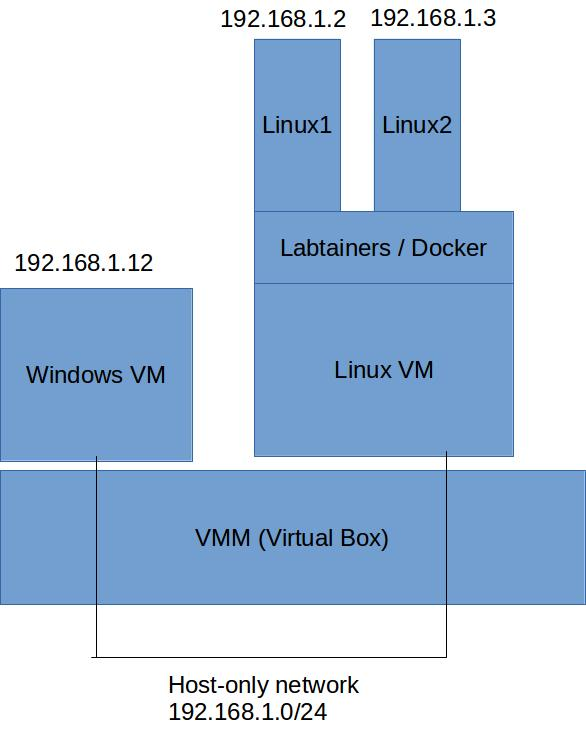
\includegraphics[width=0.4\textwidth]{ExternalNetworks.jpg}
\caption{Networking with external hosts.}
\label{fig:external hosts}
\end{figure}

Also see the description of Multi-user labs in \ref{multi user}.

\subsection{Network interface assignments}
Docker appears to assign network connections to containers in alphabetical order.  E.g., connecting
networks LAN1 and LAN2 to a container would result in LAN1 being connected to device eth0 -- regardless
of the order in which LANs are defined within the start.config file.  Understanding this ordering may
be helpful for networking labs, e.g., when defining routes.

\section{Building, Maintaining and Publishing Labs} \label{publishing}
This section describes how labs are built, maintained and published.  Additional information
on tools and strategies intended for use by outside developers are described in section \ref{imodules}

Typically, when a Labtainer is started, the container's associated Docker images are pulled from
the Docker Hub if they are not already local on the Linux host.  When building and editing labs,
the designer desires to run images reflecting recent changes that have been made.  The framework
includes logic to identify dependencies within containers whose image content has changed, 
and it will rebuild those images, (using the Docker build command).  The framework will only 
rebuild those images that have changed.  The designer can force the rebuild of all images within
a lab by appending the ``-f'' switch to the end of the ``rebuild.py'' command.  That switch is not
intended for routine use because it wastes time and masks errors in our dependency logic.

If you build a new Labtainer exercise, the container images will not be on the Docker Hub unless you put
them there.  If you
create your own public repository on the Docker Hub (https://hub.docker.com/), you can populate that
with your lab(s) by setting the ``REGISTRY\_ID'' value in the start.config file for the lab(s). You
would then use the distrib/publish.py script to build, tag and push your lab container images to your registry.
Please refer to the section \ref{imodules}.

\subsection{NPS Development Operations}
When building lab images at NPS, please set the LABTAINER\_NPS environment variable to "YES", e.g.,
\begin{verbatim}
   export LABTAINER_NPS=YES
\end{verbatim}
This will force packages to be retrieved from the local NPS mirrors (centosmirror.uc.nps.edu or
ubuntumirror.uc.nps.edu).  Refer to section \ref{package sources} for additional information.
If builds fail with this environment set, it is likely due to trying to install packages not present
in the mirror.  In those cases, edit the Dockerfile to remove this line:
\begin{verbatim}
ENV APT_SOURCE $apt_source
\end{verbatim}
\noindent That will force use of the original apt-sources for that container.

Labs must be checked into the local Git repository in order to be distributed.  After creating and testing
a new lab, use the scripts/designer/bin/cleanlab4svn.py script to remove temporary files that do not belong in 
git.  Use the publish.py script (described above) to publish the lab containers.
The distrib/mkdist.sh script is used by NPS to create the distribution tar file.  This script relies on
your local Git repository as the source to the Labtainer scripts and labs.  Use the mk-devel-distrib.sh script
to publish the developer configuration of the tar file.  

The mkdist.sh and mk-devel-distrib.sh scripts include "myshare" variables that define a path to a directory
shared with the development VM's host. The scripts will place the resulting tar files in this directory.  You
must then manually transfer the updated tar files (including the {\tt labtainer\_pdf.zip} file) to the Liferay
server at
\begin{verbatim}
davs://my.nps.edu/webdav/c3o-staging/document_library/labtainers
\end{verbatim}
After transfering the files, use the Liferay ``Publish to Live'' function to make the files available on the
Labtainers website (which is also where they are pulled from when a student runs update-labtainer.sh).

Be sure to push your Git repository updates to the GitHub master.

The distrib/publish.py script is used to rebuild and 
publish individual labs, or optionally all of the Labtainer exercises managed by NPS.
The publish.py (without the {\tt -l} option) script will only rebuild labs that have changed.  After pushing a new lab container
image to the Docker hub, the script deletes the image from the local system.  The intent is to
ensure that future testing of the lab is done on the authoritative copy, i.e., from the hub.

Labtainer base images are built and published from the scripts/designer/bin directory.  Prior to publishing
baseline images, it is suggested that all local images be purged from the development machine, e,g.,
\begin{verbatim}
    /trunk/setup_scripts/destroy-docker.sh
\end{verbatim}
\noindent This will ensure that new baseline images do not incorporate layer remnants.

All new images should be first built and pushed onto the test registry, i.e., using the 
{\tt ./publish\_image.sh <image> -t}

Framework modifications made to support changed or new functions within container images
must be evaluated with respect to their impact on compatibility. If a new lab image requires
an updated Labtainers framework, then the "framework\_version" must be incremented within the
bin/labutils.py script \textbf{before} the image is built and published.  This will prompt users
to run update-labtainer.sh prior to running any newer lab image. 
Also insure that these lines are present in the container dockerfile:
\begin{verbatim}
ARG version
LABEL version=$version
\end{verbatim}
\noindent And, be sure to publish the revised framework before publishing the revised lab(s).

\subsection{Alternate registry for testing}
If the environment variable {\tt TEST\_REGISTRY}, is set to TRUE, labs to be pulled and pushed
into an alternate registry defined in the trunk/config/labtainer.config file test\_registry entry.
Also, the {\tt build\_lab.py}, {\tt labtainer}, and {\tt publish.sh} scripts include {\tt -t} flags to
force the system to reference the test registry instead of the Docker Hub.
It is easy to set up a registry (it is a container!), \url{https://docs.docker.com/registry/deploying/}
Use the {\tt trunk/setup\_scripts/prep-testregistry.sh} script to
prepare a test system to use a test registry.

\subsection{Large lab files}
Consider storing the authoritative source of large files (e.g., pcaps) or directories in external locations, e.g., nps.box.com.  This has two
advantages:  1) Reduces the size of the lab designer distribution tar; 2) avoids putting large files
into github.  Note this issue does not affect container images, which will always include the large files regardless of how they
are stored.  The question is simply the location of the source of the large files for purposes of
rebuilding a specific lab.   Our model is to provide potential lab developers with a distribution that is not gigabytes, but also contains
whatever is needed to rebuild existing labs -- or at least links that are automatically followed when building the lab.

A file named {\tt <lab>/config/bigexternal.txt} with entries as follows:
\begin{verbatim}
<url> <relative_path>
\end{verbatim}
\noindent will cause a rebuild to look for a file at {\tt relative\_path} relative to the lab directory, and
fetch it from the {\tt url} if it is missing.  Note that the date/times of these files are not referenced for rebuild dependencies
due to limitations in product such as box.com which fails to provide file modification times.  Instead, the modification time of the
bigexternal.txt file is used to control rebuilds.  Thus, if you update one of the large files, you will want to make a gratuitous change
to the bigexternal.txt file to force a rebuild (for you and others who may extend your lab.)

\subsubsection{Reuse of large file sets}
\label{manifest}
The use of ``sys\_tar'' and ``home\_tar'' described in \ref{large files} facilitates sharing of common
baselines of large or numerous files.  New labs can incorporate tar files from existing
labs through the use of ``external-manifest'' files, (see the xsite/victim/home\_tar as
an example).   The syntax of the external-manifest is shown below, and it may contain
multiple entries, one per line:
\begin{verbatim}
lab:container
\end{verbatim}
\noindent Where ``lab'' is the name of the lab, and ``container'' is the name of the container
whose tar file is to be included.

The framework will include content of tar archives referenced within these files
when creating an archive for the new lab.  This allows the sys\_tar to include lab-specific files
as well as files from other labs.  Designers should avoid adding duplicate tar files to the SVN repository.
This will avoid duplication of the files when a new distribution is created.

\subsection{Package sources for apt and yum}
\label{package sources}
Labtainer base images include configuration files to use local NPS mirrors when creating derivative
images.  The original apt or yum sources are restored to an image if it is built without an environment
variable of {\tt LABTAINER\_NPS=YES}  The original sources are also restored when any container is first
run.  See the baseline Labtainer Dockerfiles in {\tt trunk/scripts/designer/base\_dockerfiles} to understand
how the sources files are manipulated.

The {\tt apt\_source} entry in the trunk/config/labtainer.config file will set the {\tt \$apt\_source}
environment variable in a Dockerfile, and this can be used by lab designers to force image builds to use
alternate sources.  By default, the value of the variable is ``archive.ubuntu.com''.  This hostname can be 
overridden via the trunk/config/labtainer.config file apt\_source entry, and having the following in your Dockerfile:
\begin{verbatim}
RUN sed -i s/archive.ubuntu.com/$apt_source/ /etc/apt/sources.list
\end{verbatim}

\subsection{Locale settings}
The locale settings, (e.g., used when interpreting character encodings) are set to en\_US.utf-8 
as can be seen in 
\begin{verbatim}
trunk/scripts/labdesigner/base_dockerfiles/Dockerfile.labtainer.base
\end{verbatim}
Similar Dockerfile entries in new or existing labs can provide alternate locale settings.

\subsection{Lab versions}
Substantive changes to an existing published lab should be made in
a new named lab.  A \textit{substantive} change is defined as one that would
break any existing installation in a manner that could not be corrected
with a framework update.  Issues with compatibility between two
lab versions is often due to there being lab-specific files on the framework,
(i.e., from where the lab is run) as well as within the Docker images that
make up the lab.  When a newer version of a lab image is published, it must 
be able to work with existing installations.  If that requires an update to the
framework, then that update cannot break any existing labs present in that
installation, i.e., labs that have already been started.

For example, \textbf{never} change container names for existing labs.  If such
a change is needed, create a new lab, and assign version numbers to
it and the old lab.  

Lab version numbers are kept in the optional {\tt labs/[lab]/config/version} file.
There is no need to have such a file until there are two or more versions of the
same lab.  (Note if you want two versions of a given lab to be runnable and to appear
in the list of labs, then they are not versions of the same lab.  They are different
labs.)  The format of a lab version file is:
\begin{verbatim}
    lab-base version
\end{verbatim}
where {\tt lab-base} is a name to associate with the multiple versions.  It can be
anything and does not appear at the user interface.  The {\tt version} is an integer.

To create a new version of a lab:
\begin{itemize}
\item Create a new lab using {\tt new\_lab\_setup.py} (perhaps with the clone option).
\item Create a version file for the old lab (if it does not already have one). 
\item Create a version file for the new lab, giving it a version numerically greater than
the old version.
\item Add the old lab name to the trunk/publish/skip-labs list.
\end{itemize}

When the user types the {\tt labtainer} command with no arguments, the list will then
only include the latest version of that lab.  An exception is if the old lab already
has been run in this installation, in which case both lab versions will display.

\subsection{Creating new base images}
Labtainer base images are managed using scripts and configuration files in the {\tt scripts/designer} directory.
The {\tt bin} subdirectory includes a set of scripts that create various base images, and the
{\tt base\_dockerfiles} contain their Dockerfiles.  Use those as a template.

Typically, new base images are created to support a new lab.  Proper Labtainer lab Dockerfiles have {\tt FROM} directives
that include the {\tt \$registry/} qualifier, however your new base image might not yet be published to a registry
as you test it, and tagging the new base image with the registry name may complicate your desired workflow.  
Use the {\tt -L} option to the {\tt rebuild} command to direct the build to use unqualified image names if needed.

\subsection{Importing labs: Warning!}
\label{warnings}
Avoid the use of ``shared folders'' in VMWare and VirtualBox as a means of copying lab
directories.  Use tar and/or scp instead.  Otherwise permissions of directories may
be changed, e.g., no x access to /etc for other.


\section {Labtainer Instructor Modules (IModules)}
\label{imodules}
This guide describes how instructors can add content to Labtainers.
Instructors extend Labtainers with new labs or customized versions of existing
labs by defining IModules and directing their students to enable the IModules within
their individual Labtainers instances.\footnote{Or, instructors can enable IModules in VMs, and direct students to use those.}
Students simply type: {\tt imodule <path>} to add a given URL to their Labtainers instance.
The scope of instructor-generated extensions can range from modified lab manuals 
to new Labtainer exercises.  The Labtainers framework provides tools
to assist instructors in creating and publishing these extensions. 

\subsection{Labtainers distribution strategy}
To understand how IModules are distributed, it is helpful to first review the general
Labtainers distribution strategy.  A Labtainers installation, (e.g., the initial content of a Labtainers VM 
appliance, or the results of installing from the distribution),  includes the scripts and configuration files 
needed to run all Labtainers exercises.  The installation initially only includes a small number of 
Docker container images that provide the core of container images for each of the labs.   
When a student first starts a given lab, the framework retrieves all Docker image layers 
required for that lab.  These layers are retrieved from the Docker Hub, and build upon the core images
present in the initial distribution.   The scripts and configuration files are 
published as a tar archive on the Labtainers website.  Whenever a Labtainers installation is updated, 
the archive is retrieved from the website and used to update the installation.

Files needed to create Docker images are typically not distributed in Labtainers distributions, but are 
installed when the user runs the update-designer script.  These files are drawn from a separate 
tar archive on the Labtainers website.  

\subsection{Imodule distribution strategy}
Instructors place archives on a web server and student
instances of Labtainers retrieve those archives from the web server while retrieving other
Labtainer updates.  When creating new labs, instructors publish the lab Docker images to
DockerHub, where they'll be retrieved by the framework when students run that lab.
While the publishing of extensions does not depend on any particular 
source control system, supporting tools that simplify archive creation are built around git.  

Archives published by instructors are tar files that include only changed and new files,
relative to the Labtainers baseline.  Inclusion of unchanged (relative to the 
Labtainers baseline) files is discouraged, as is publishing only deltas from previous
IModule publications.  Put another way, an IModule will contain any 
and all files
necessary for running, (not building), all new labs -- or to modify existing labs, 
relative to the Labtainers baseline as defined by the GitHub master repository.

Support tools simplify creation of IModule tar files through use of git attributes.
Instructors who chose not to use git are responsible for creating a tar of selected
files -- which may be trivial, e.g., if the IModule consists of lab manual modifications
or new lab guides.  Paths within tar files will be relative to the labtainers/lab
directory.  For example, a revised telnet-lab manual would have the path:
\begin{verbatim}
telnet-lab/docs/telnet-lab.pdf
\end{verbatim}
\noindent Note the modified source, e.g., docx files, need not be included in the IModule
archive, though the support tools do include them.

Typically, each participating instructor will publish a single archive (i.e., a tar file)
at a publically accessible URL specific to the instructor or institution. The URL 
is distributed to students and entered into their Labtainers 
instance using the {\tt imodule} command \footnote{The full URL is published because many
web hosting systems, e.g., box.com make it impossible to construct URLs from relative paths}.  
For example, if the instructor publishes
at \url{https://myschool/mystuff/labtainers/imodule.tar}, the students would each issue
this command to Labtainers:
\begin{verbatim}
imodule myschool/mystuff/labtainers/imodule.tar
\end{verbatim} 

The student labs will be updated to include those IModules the next time the student runs
either {\tt update-labtainer.sh} or {\tt imodule -u}.

IModule support tools rely on instructor contributions existing in local git repositories.
The tools do not reference remote repositories.  IModule repositories have no relationship
to the main Labtainers repository, and should be managed within Labtainer
distributions rather than within local repo copies of the main Labtainer repository.   \footnote{In general,
instructors and lab designers are encourage to work from Labtainer distributions rather
than repos pulled from the Labtainers repo at GitHub to avoid git repository conflicts.}

\subsection {Custom lab manuals}
The easiest way to provide your students with a custom version of a lab manual that they can reference from Labtainers
is descrbed below.  This does not require that you use the Labtainer VM or git. The example assumes you are customizing
the telnet-lab manual.
\begin{itemize}
\item Create your version of the manual in the pdf format (if the manual source is docx, export it as pdf).
\item Put that manual in a file with the original name, in a directory whose name is the lab, e.g.,
\begin{verbatim}
    telnet-lab/telnet-lab.pdf
\end{verbatim}
\item Create a tar file of the manual including the lab name in the path.
\item Publish that tar file onto a web server, i.e., something that responds to {\tt http get} commands.
\item Instruct your students to provide that URL to the {\tt imodule} command. 
\end{itemize}
If you wish to publish multiple custom lab manuals, put them all in the same tar file.
\subsection {Imodule examples}  
These examples assume the instructor is working from a Labtainers distribution, e.g., one
of the VM appliance.
\subsubsection {Modify a lab manual for the telnet-lab}
In this example, the instructor wants his or her students to work with a customized version
of the telnet-lab manual.  
\begin{itemize}
\item Change directory to labtainer/labs
\item Initialize the git archive: 
\begin{verbatim}
git init  
\end{verbatim}
\noindent (Do this only once, no need to repeat for each IModule.)
\item Add the original Labtainer file as the baseline: 

\begin{verbatim}
git add telnet-lab/docs/telnet-lab.docx
\end{verbatim}
\item Edit the telnet-lab/docs/telnet-lab.docx file
\item Commit your change: 
\begin{verbatim}
    git commit telnet-lab/docs/telnet-lab.docx
\end{verbatim}
\end{itemize}

This change has no effect on any Docker container, so we need only generate the 
updated tar:
\begin{verbatim}
    create-imodules.sh
\end{verbatim}

\noindent Then publish the imodule.tar to the website.

\subsubsection{Create a new lab}
In this example, the instructor wants to create a new lab for use by his or her students.
This example assumes the instructor has created a DockerHub registry that is publicly accessible.
\begin{itemize}
\item Change directory to labtainer/labs
\item Initialize git archive: git init  (Do this only once, no need to repeat for each IModule.)  
\item Create the lab per the Lab Designer User Guide, for this example, we assume the lab is my-new-lab.
\item Include the name of your DockerHub registry the lab config/start.config file.
\item Complete development and testing of the lab, e.g., build a SimLab test.
\item While in the my-new-lab directory, run {\tt cleanlab4svn.py} to remove temporary files that should not be under source control.
\item While in the lab directory (parent of my-new-lab), add the lab to source control:
\begin{verbatim}
    git add my-new-lab
    git commit my-new-lab -m "Adding an IModule"
\end{verbatim}
\item Publish the lab container images: 
\begin{verbatim}
    ./publish.py -d -l my-new-lab
\end{verbatim}
\noindent This will rebuild the lab container images and publish them to your DockerHub registry.  Note the {\tt -d} option directs the 
function to publish to the DockerHub registry named in your lab start.config file.  Otherwise, it will try to publish to a test registry.
Use of test registries is optional, and are described in the \textit{Lab Designer User Guide}.
\item Generate the updated IModule tar:
\begin{verbatim}
    create-imodules.sh
\end{verbatim}
\item Then publish the imodule.tar to your website.
\end{itemize}

\section {Remote access and control of Labtainer exercises}
This section describes features intended for use within structured environments in which one or more students are performing 
a lab exercise under supervision of an instructor or red-team member.  This does not apply to environments in which students 
individualy run Labtainers on dedicated computers at their own pace. 

The environment may have one of two forms:

\begin{enumerate}
\item Each student has a dedicated computer upon which a Labtainer VM resides, and the instrutor has network access to each computer; or,
\item Multiple Labtainer VMs (or custom-built VMs containing Labtainers) run on one or more servers that are networked together.  
Students interact individually with their allocated VM using a tool such as VMWare Horizon or Apache Guacamole, 
which presents the student with the Linux desktop of their allocated VM via a browser or client application.
\end{enumerate}
\noindent We assume that something within the infrastructure allows remote network access by an instructor to each VM, e.g.,
via port forwarding.  The instructor will use this network access to manage aspects of the lab exercise, and/or remotely access
selected containers, e.g., as a red-team activity.

\subsection{Remote management}
Labtainer remote management functions allow instructors to query and change the state of the Labtainers exercise 
currently running on each VM.  The remote access functions available to instructors currently include:
\begin{itemize}
\item \textbf{status} -- Display the name of the lab running on a specific VM.
\item \textbf{copy} -- Copy files into a Labtainer container per a copy directive defined in:
\begin{verbatim}
  <lab>/config/copy.config} 
\end{verbatim}
\end{itemize}

\subsubsection{File copying}
\noindent The {\tt copy.config} file contains one or more directives, one per line as follows:
\begin{verbatim}
    <directive> <container> <source> <destination>
\end{verbatim} 
\noindent Where:
\begin{itemize}
\item \textit{directive} is a arbitrary string identifier that names the directive.
\item \textit{container} is the name of the container into which the files are to be copied.
\item \textit{source} is a source path upon the VM.  If this path starts with {\tt \$LAB}, the path is relative to
the lab directory.  Otherwise, a full pathname is expected, e.g., the path to a folder shared with all VMs on a host.
\item \textit{destination} is the destination path upon the target container.  Permissions are retained if possible, e.g, if the
source files are owned by {\tt root:root}, that will be maintained on the destination.
\end{itemize}
\noindent The semantics of source and destination are per the Unix {\tt cp -a} command.  Please see the discussion of {\tt SRC\_PATH} 
and {\tt DEST\_PATH} in \url{https://docs.docker.com/engine/reference/commandline/cp/}

\subsubsection{Client and server setup}
The python service at {\tt scripts/remote/remote.py} should be started on each Labtainers VM with the {\tt --daemon} option.

The python client at {\tt host\_scripts/remote/remote.py} should be copied to whatever host the instructor will work from.

Port forwarding for each VM should be defined such that some host port is forwarded to port 60000 on the VM.  You would assign
each VM on a given host a different host port number. That host port number will be how the instructor names different VMs on the same host.
For example, on VirtualBox, the port forwarding entry for one VM might look like:
\begin{verbatim}
   Host IP     Host Port   Guest IP  Guest Port
   0.0.0.0     60003       0.0.0.0   60000
\end{verbatim}

Then, if the instructor is working from the computer that hosts the VM, the following command would cause a copy 
directive named {\tt one} to occur on that VM if it is
running a lab named {\tt tlab}:
\begin{verbatim}
    ./remote.py -l tlab -c one -p 60003
\end{verbatim}

\subsection{Remote access to containers}
This section describes environments in which an instructor or red team member is to interact with containers within the lab,
e.g., to perform penetration testing.  This interaction would occur via computers external to the lab exercise, e.g., networked
to a server hosting VMs.  The strategy employed to achieve this depends on whether the lab utilizes GNS3, (which manages the virtual
networks without relying on Docker networking).

\subsubsection{Remote access without GNS3}
Docker port publishing provides external network access to containers.
For example, remote ssh access to a specific container within the lab can be achieved as follows:
\begin{itemize}
\item Use the {\tt PUBLISH} directive in the start.config to bind a container port to a host VM port, e.g.,
\begin{verbatim}
    PUBLISH 0.0.0.0:60020:20/tcp
\end{verbatim}
\item Use port forwarding to bind the VM port to a server port.  Here, the host port would differ for each VM on a server as a
means of naming the VM whose lab is to accessed.  For example, on VirtualBox, a port forwarding entry might be:
\begin{verbatim}
   Host IP     Host Port   Guest IP  Guest Port
   0.0.0.0     61022       0.0.0.0   60022
\end{verbatim}
\end{itemize}

\noindent The above example would then allow an external computer to ssh into the selected container using port 60122,
assuming the container has SSH enabled (see the telnet-lab server container for an example).  Authentication to control who can SSH
into a given container could be provided through use of SSH keys.  This remotely accessed container can be hidden from the student, and provide
the instructor or red-team participant with a means to probe and attempt to compromise the other computers within the Labtainers exercise network.

\subsubsection{Remote access with GNS3}
For labs that run in the GNS3 environment, remote network access is provided through use of the GNS3 \textit{cloud} 
endpoint device, which interacts with an Ethernet network interface.  In this example, access is provided from external to
the VM -- with no network access to the container from within the VM.

The following assumes your VM has a virtual Ethernet interface named {\tt enp0s3}, with IP an address  on the
{\tt 10.0.2.0/24} subnet.  On your VM, find the Ethernet interface that has an assigned IP address. 
Alternately you could define the VM to share a physical host network, but that is outside the scope of this example.

Define a component within your Labtainers lab that is be remotely accessed, e.g., a workstation or router, and assign it an IP
address on the {\tt enp0s3} interface subnet, e.g., {\tt 10.0.2.100}.  Within the start.config file, provide the container with
the {\tt KICK\_ME <LAN>} attribute, where LAN is the name of the network intended to be connected to the cloud component.  Then, 
when defining the GNS3 network topology, i.e., creating and connecting links: 

\begin{itemize}
\item Select a {\tt Cloud} component from the {\tt Browse End Devices} menu, and drag it to the desktop.  
(computer terminal icon).
\item Right click, select {\tt Configure} and confirm that the Ethernet interface that you selected (e.g., enp0s3) is in the list.
If it is not there, select the device from the pull-down list and click the {\tt Add} button.  Then click {\tt OK}.
\item Use the network links to connect the cloud to the desired component.
\item Use port forwarding as described earlier to map host ports to ports on the VM.  When defining port forwarding, enter 
{\tt 0.0.0.0} as the ``Host IP'', and the container IP address, e.g., {\tt 10.0.2.100} as the ``Guest IP''.
\item You should now be able to ssh to the container from outside of the VM using the mapped port.
\end{itemize}


Alternately, to provide access from the VM (but not from external sources), pick virbr Ethernet interface and:

\begin{itemize}
\item Select a {\tt Cloud} component from the {\tt Browse End Devices} menu, and drag it to the desktop.  
(computer terminal icon).
\item Right click, select {\tt Configure} and delete the default Ethernet interface if any is selected.
\item Click the {\tt Show special Ethernet interfaces} checkbox in the lower left.  That should add devices to the pull-down
list.
\item Select the {\tt virbr0} device from the pull-down list and click the {\tt Add} button.  Then click {\tt OK}.
\item Use the network links to connect the cloud to the desired component.
\item When the lab is started, you should be able to ping the connected container from the VM.
\item Use port forwarding as described earlier to map host ports to ports on the VM.  When defining port forwarding, enter the
container IP address as the ``Guest IP''.
\end{itemize}
Note that the subnet used for this remote access is defined by the VM's Ethernet device.  Putting multiple lab computers
on that subnet as part of the lab network topology may be awkward and confusing to students since 192.168 addresses are
private.  

When a GNS3 Labtainer is run with the {\tt --student} option, the Cloud components are hidden, as are any Labtainer
components whose {\tt start.config} entries include {\tt HIDE YES}.  Links to hidden devices are also hidden.

\section {Multi-user Labtainers}
\label{multi user}
Labtainer exercises can support multiple concurrent users, such as students collaborating or competing on a shared 
set of networked components.  A multi-user lab can be operated in any one of three modes:
\begin{enumerate}
\item Dedicated to a single student, e.g., on a laptop or a VM allocated to the student from a VM farm.
\item Shared by multiple students, each running Labtainers on a per-student VM with shared componets running on separate
Labtainers VM.  This is illustrated in Figure \ref{fig:multi-multi}
\item Shared by multiple students, each SSHing from a non-Labtainer VM into a per-student Labtainer computer on a single
VM running Labtainers.  This is illustrated in Figure \ref{fig:multi-single}
\end{enumerate}

\begin{figure}[H]
\centering
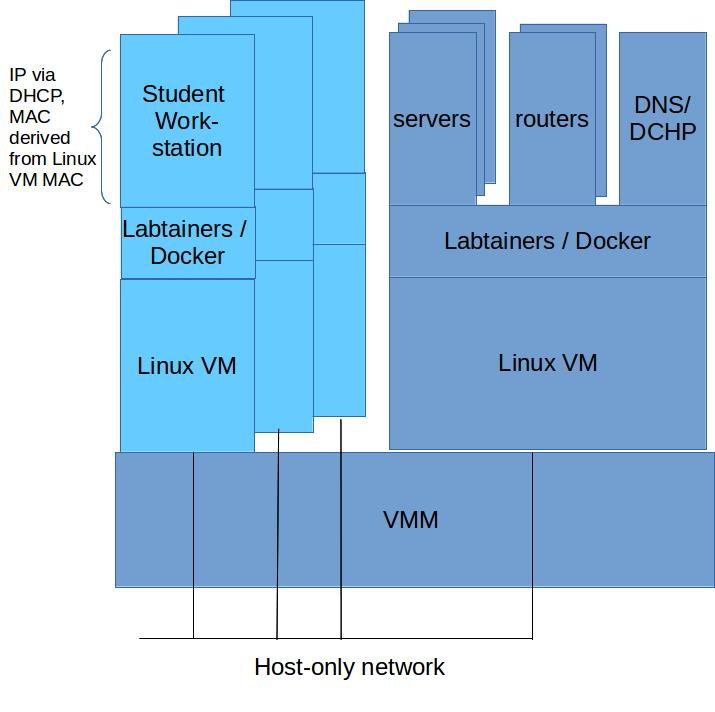
\includegraphics[width=0.4\textwidth]{multiuser-multilabtainers.jpg}
\caption{Multi-user Labtainers with multiple instances of Labtainers.}
\label{fig:multi-multi}
\end{figure}

\begin{figure}[H]
\centering
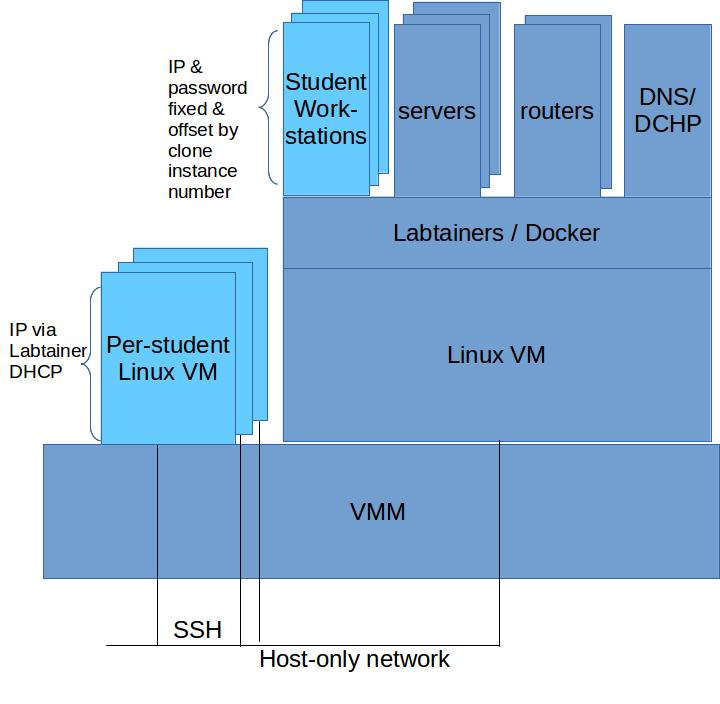
\includegraphics[width=0.4\textwidth]{multiuser-onelabtainer.jpg}
\caption{Multi-user Labtainers via SSH.}
\label{fig:multi-single}
\end{figure}

Both of the multiuser modes require a host-only network defined by the VMM.  This network should be defined
before it is allocated to any VM, and the DCHCP server on the host-only network should be disabled within 
the VMM.  

\subsubsection {Multi-user Labtainers, one Labtainer VM per student}
In this approach, each student is assumed to have been allocated an
individual VM upon which Labtainers is installed.
The student has access to that VM, e.g., via ssh or a vSphere client.  
Each student VM runs a single per-student workstation Labtainer component.
The remaining containers, e.g., vulnerable servers, all run on a single VM,
which we refer to herein as the ``server VM''.  Provisioning a lab to run
in this mode is summarized below.

\begin{itemize}
\item Allocate the host-only network to each Labtainers VM.  Be sure
to disable the IPv4 networking for this network on each Labtainers VM, and
set the network interface to promisuous mode (within the Linux host as well).
For example:
\begin{verbatim}
    sudo ifconfig ethx 0.0.0.0
    sudo ifconfig ethx promisc
\end{verbatim} 

\item Start the lab on the server VM using the labtainer command with the --server (-s) switch. This
causes Labtainers to start each container in the lab that is not tagged as a ``CLIENT''. 

\item Students then
start the lab on their individual VMs using the labtainer command with the --workstation switch, which will cause
the student VM to only start the container identified as the ``CLIENT'' in the start.config file.
\end{itemize}

When conformant labs (see \ref{conformant multi-user}) are started, the workstation containers 
use DHCP to optain IP addresses from a Labtainers DHCP server.  The MAC address of the workstation
container is derived from the MAC address of the Linux VM host-only network interface (to avoid
duplicate MAC addresses on the host-only network). 

\subsubsection {Single Labtainers VM with multiple students}
In this approach all the Labtainer containers will run on a single VM.  
Students have access to one or more other
VMs hosted on the same VMM as the VM that hosts Labtainers. Students will SSH from these VMs into the container workstation
allocated to the student via the host-only network.  The ssh command may include the ``-X'' option to permit X11 forwarding, thus allowing students to
run GUI-based applications on their workstation containers.

\begin{itemize}
\item Allocate the host-only network to the Labtainers VM. Be sure
to disable the IPv4 networking for this network on the Labtainers VM, and
set the network interface to promisuous mode (within the Linux host as well).
\item Allocate the host-only network to each VM used by students to SSH into their
Labtainers workstation.  Configure the network on the VM to use DHCP (the host-only
DHCP server should be disabled, the VM will get an IP from a Labtainer DHCP server.)

\item Start the lab on the server VM using the labtainer command with the --clone\_count (-n) switch,
specifying the quantity of per-student client containers to start.

\item Students then ssh into their respective containers over the host-only network.
\end{itemize}

Conformant labs will assign each student workstation component an IP address in a sequence,
starting from a fixed value.  These IP addresses are allocated to the students.

\subsection{Creating conformant multi-user labs}
\label{conformant multi-user}
The following suggestions are intended to yield labs that can be started in any of
the three operating modes.

\begin{itemize}
\item The lab should include a ``client subnet'' via which multiple VMs will communicate.

\item Within the {\tt start.config} file, identify this subnet as either a MACVLAN or
a MACVLAN\_EXT.  The MACVLAN\_EXT
option will create a MACVLAN for this interface regardless of what mode the lab is started in,
and is only intended for use if the lab includes an external host as described in \ref{external hosts}.

\item Itentify the client component within the {\tt start.config} file using:
\begin{verbatim}
    CLIENT YES
\end{verbatim}

\item Define the client component network address for the client subnet using the
{\tt +CLONE\_MAC} option, e.g., 
\begin{verbatim}
    LAN 192.168.1.10+CLONE_MAC
\end{verbatim}
\noindent  When run in single user mode, the {\tt +CLONE\_MAC} suffix is ignored.  When run
with multiple Labtainer instances, the last four bytes of the network MAC address for
each client is cloned from the network interface tied to the MACVLAN.  When all multi-user
Labtainer workstations run on a single VM, then the IP address is incremented by one less
than the clone instance number.

\item Include a dhcp server as one of your containers, e.g., per the dhcp-client lab.  
The labtainer.network base includes the dnsmasq service, which includes a DHCP
server.  Reconfigure dnsmasq to start the DHCP service, e.g., in your fixlocal.sh script.
\item Edit the dhcp container's {\tt \_system/etc/dnsmasq.conf} file to include the
range of DHCP addresses you wish to allocate to the clients.  When multiple instances
of Labtainers are run, then ``client'' is the per-student Labtainer workstation.  When
there is a single Labtainers VM, then ``clients'' are the VMs from which students
SSH into their Labtainer workstations.  An example dnasq.conf entry is:
\begin{verbatim}
    dhcp-range=192.168.1.10, 192.168.1.99, 12h
\end{verbatim}


\item Enable dhcp on the client workstation components by installing isc-dhcp-client
(via the Dockerfile), and putting this in the workstation \_system/etc/rc.local:
\begin{verbatim}
/sbin/dhclient-labtainer eth0
\end{verbatim}
\noindent Note the dhclient-labtainer invokes the dhclient program and then
manually sets the ip address.  This is a workaround for a Docker limitation.

\item Include an SSH server in the workstation container, e.g., by deriving it from the labtainer.network base.
Include a {\tt \_system/etc/ssh/sshd\_config} file for the workstation container that permits X11 forwarding (if desired),
e.g., by copying the file from the kali-test lab.

\item Password management (only has an effect in multiuser mode when all Labtainers components are on a single VM). 
Assuming you'd like to allocate each student a unique (insecure) password for purposes of
further ensuring one student does not accidently ssh into some other student's workstation, put
this in the workstation's \_bin/fixlocal.sh file:
\begin{verbatim}
    newpwd=studentCLONE\_NUM
    user=$2
    /usr/bin/passwd $user <<EOF
    $1
    $newpwd
    $newpwd
    EOF
\end{verbatim}

\noindent Add, this in the labs/[your lab]/config/parameter.config
\begin{verbatim}
PASSWD : CLONE_REPLACE : .local/bin/fixlocal.sh : CLONE_NUM : CLONE
\end{verbatim}

\end{itemize}

\section{Limitations} \label{limitations}
The labtainers framework limits labs to the Linux execution environment.
However, a lab designer could prescribe the inclusion of a separate
VM, e.g., a Windows system, and that VM could be networked with the Linux
VM that hosts the Docker containers as described in \ref{external hosts}.  
Future work would be necessary to include
artifacts from the Windows system within the framework's automated assessment
and parameterization.

The user does not see the /etc/fstab file.  Only virtual file systems can be
mounted (or those mounted when the container is created.)

Kernel logs do not appear in {\tt /var/log/kern.log}.  For logging events
such as iptables, consider using ulogd and a ``NFLOG'' directive in place of
a ``LOG'' directive.  See the dmz-lab as an example.

The available Docker network drivers do not permit IP address overlap between virtual networks.
For example, you cannot define two 192.168.1.0/24 LANs.

Student use of the shell directive "source" will cause stdin/stdout to not be captured.

Inquisitive students will see evidence of artifact collection.  Home directories
on containers includes a \texttt{.local} directory that includes Labtainer scripts that manage
capturing and collection of artifacts, and that directory contains the stdin and
stdout files generated by student actions. Additionally, when the student starts a process
that will have stdin and stdout captured, the student will see extra processes within
that process tree, e.g., the \texttt{tee} function that generates copies of those data streams.
All of the containers share the Linux kernel with the Linux host.  Changes to
kernel configuration settings, e.g., enabling ASLR, will be visible across all
of the containers.


\section{Notes} \label{Notes}
\label{Notes}
\subsection{Firefox}
\subsubsection{Profile and configuration changes}
The labtainer.firefox image includes a /var/tmp/home.tar 
which is expanded into the user home directory when parameterize.sh is run.
This tar includes a profile in .mozilla that avoids firefox starting with its 
welcome pages and privacy statements.  The labtainer.firefox image includes a 
customized /usr/bin/firefox that starts the browser in a new instance so it does 
not share existing browsers.  The {\tt about:config}
was altered to disabled insecure field warnings for the labs that do not use SSL connections to web servers.

\subsubsection{Browser history}
If you wish to assess places a browser has visited, e.g., use a pregrade.sh to extract sites from the
firefox places.sqlite file, put {\tt places.sqlite} into the lab's /\_bin/noskip file.

\subsubsection{Slow browser startup}
Some html, e.g., for the softplc, want to visit fonts.googleapis.com.  If no gateway/dns is available, there is a long timeout.
Try adding 
\begin{verbatim}
ADD-HOST fonts.googleapis.com:127.0.0.1 
\end{verbatim}
\noindent to start.config to avoid the timeout.

\subsubsection{Crashes in SimLab}
See \ref{simlab_notes} for information on avoiding firefox crashes when it is restarted in SimLab.

\subsection{Wireshark}
Wireshark will not run as root in Labtainer containers.  
The wireshark installion in the labtainer.wireshark image is configured to not
require root to collect network packets:

When using the wireshark image, after the existing 
\begin{verbatim}
RUN adduser $user_name sudo
\end{verbatim}

\noindent add:

\begin{verbatim}
RUN adduser $user_name wireshark
\end{verbatim}

\subsection{Elgg}
The xsite/vuln-site/myelgg.sql file needs to be loaded for elgg to run.  First edit it to
change xsslabelgg.com to your site name (two changes).  Copy the sys\_tar/var/www/xsslabelgg.com/elgg
to your new lab.  Note the elgg/views/default/output files have been modified to permit cross site scripting.
\subsection{Host OS dependencies}
On rare occations, performance of a lab may depend on the host Linux OS.  An example is some
kernel tuning parameters viewed and set via sysctl are not visible within containers on eariler versions
of Ubuntu.  If your lab has such OS dependencies, you can check the OS and warn the student/instructor via a script
named "hostSystemCheck.py" placed withe the \_bin directory of any of the lab's containers.  This script shall
return the value '0' if dependencies are met, and '1' if dependencies are not met.  In the latter case, the 
startup.py will prompt the use to continue or abort.  Your script should explain the situation to the student.
An example of such a script is in the labs/tcpip/server/\_bin directory.
\subsection{Login Prompts}
See the centos-log lab for an example of a lab that prompts users to login to the virtual terminal.
In particular, you will need the {\tt bin/student\_startup.sh} script, and the {\tt \_system/sbin/login} program and the {\tt \_system/etc/login.defs} and {\tt securetty} files.

\subsection{Networking Notes}
\label{Networking Notes}
\subsubsection{SSH}
The labtainer.network baseline Dockerfile includes the following:
\begin{verbatim}
ADD system/var/run/sshd /var/run/sshd
RUN sudo chmod 0755 /var/run/sshd
\end{verbatim}

For containers derived from the kali base, and others non-labtainer bases, use this line in your dockerfile
to enable ssh into the box.
\begin{verbatim}
RUN sed -i 's/UsePAM yes/UsePAM no/' /etc/ssh/sshd_config
\end{verbatim}
\subsubsection{X11 over SSH}
The scripts/designer/system/etc/ssh/sshd\_conf allows X11 tunneling over ssh, e.g.,
from a remote VM connected to the same host-only lan as a container running the GUI
application.  Use {\tt ssh -X container\_ip} to enable X11 tunneling in the ssh session.

\subsubsection{Traffic mirroring}
Send copies of traffic from one ethernet port to another using the iptables TEE operation, e.g.,
\begin{verbatim}
    iptables -t mangle -A PREROUTING -i eth1 -j TEE --gateway 172.16.3.1
\end{verbatim}
\noindent will send copies of all incoming traffic on eth1 to the component with address 172.16.3.1.
Note that gateway must be a next hop, or you will have to configure the nexthop to forward it further.
This is useful for IDS labs, e.g., snort.  Mirroring all incoming traffic into a component will let you
reconstruct TCP sessions within that component.  Mirroring output from components is not always reliable.
Besides potential for duplicate traffic, Docker networks seem to sometimes gratuitously replace destination
addresses with those of the Docker network gateway, i.e., the gateway to the host.

\subsubsection{DNS}
Install bind9 in Dockerfile.  Add zone files to /etc/bind and db files to ../\_system/var/cache/bind/.
Add reference to the /etc/bind/named.conf.local as seen in local-dns/\_bin/fixlocal.sh

\subsubsection{Overriding Docker routing and DNS}
Realistic network topologies require components to have /etc/resolv.conf and routing
table entries that do not depend on Docker gateways and related magic.  However, at some point you may
want components to be able to reach the outside world.  If you've fiddled resolv.conf and routing,
you likely broke the default Docker method for doing this.  One solution is to 
define an \textit{isp} component that has a default gateway and resolv.conf as Docker defines them.  Then
route all traffic and DNS queries to that (making use of dnsmasq and your own resolv.conf entries).  
Note you will also have to set up your own NAT on that ISP component.  See the dmz-example lab
ISP component .local/bin/fixlocal.sh as a worked example of a simple NAT setup.

As a worked example, the dmz-example lab components (other than the ISP), typically use the .local/bin/fixlocal.sh script to 
delete the Docker-generated route:
\begin{verbatim}
    sudo route del -host 172.17.0.1
\end{verbatim}
\noindent And the fixlocal.sh also replaces the resolv.conf entry with either a local DNS component, or a gateway running
the dnsmasq utility.  The /etc/rc.local script generally sets the default gateway, and configures iptables.

\subsection{User management and sudo}
The Dockerfile should make the initial user, i.e., the user named in the start.config file, a member of sudoers.
Otherwise, the fixlocal.sh script will not be unable to modify the environment.  If desired, that user can be
removed from sudoers at the end of the fixlocal.sh script.

Only the initial user (and that user's actions taken as root) are monitored.  Additional users can be added,
e.g., in the Dockerfile, but their actions are not monitored or recorded in artifacts.

\subsection{DNS fixes for rebuild problems}
\label{DNS-rebuild}
When building a container, Docker uses its Daemon's default DNS addresses, which are the external Google DNS.
Some sites disallow use of external DNS, and this results in rebuilds failing when yum/apt are unable to resolve 
host names.  The script at {\tt setup\_scripts/dns-add.sh} will update those default DNS entres to include the
DNS used by the host.

\subsection{Suggestions for Developers}
\label{suggestions}
\subsubsection{Testing assessment directives}
The result and goals configuration files can be revised and tested within a
running grader container by starting grader with the {\tt -d} option.  This saves time because you do not need to rebuild
the container for each iteration of the development of configuration files.  However,
be sure to scp the configuration files from the container to your host Linux system.  The files are in
{\tt .local/instr\_config}.  See the {tt /tmp} directory for logs.

Most result and goal assessment can occur once you have generated a suitable sample of
expected student artifacts.  In other words, adding new goal does not typically require
that you go back and re-perform student actions.  Exceptions to this are:

\begin{enumerate}
\item Adding new system commands to a ``treataslocal'' file;
\item Identifying new system files to be parsed as results.  For example, results in a log
file will not be collected unless that log file has been named in the results.config file.
\end{enumerate}

\subsubsection{3rd party applications}
Some applications that you may wish to include in your lab may already have Docker container
instances.  Bringing those into Labtainers can sometimes be challenging because such containers
often lack execution environment elements required by Labtainers for configuration steps, e.g.,
{sudo}.  Most such applications are traditional Docker images whose purpose is to package an
application.  In contrast, Labtainer Docker containers are intended to look like computers running
applications -- not as applications packaged as containers.  Is is therefore often easier, (and less
disruptive to what students see), to include the 3rd party installation procedures, (e.g., what they publish
to allow you to install their application on a Linux system), within your lab's Labtainer Docker file.

\subsubsection{Msc}
Use {\tt TERMINAL\_GROUPS} in the start.config file to organize terminals if you have more
than a few.  Otherwise the student will spend time trying to find each terminal.

\subsubsection {Docker cache}
By default, a {\tt rebuild} will make use of the Docker cache to speed up the image building process.
Use the {\tt -N} option to supress use of the cache.  This may be needed if you expect the results of
a {\tt RUN} command within a Dockerfile to change between builds.  When using the {\tt publish.py} command,
the cache is disabled by default.

\subsection {Container isolation}
Docker provides namespace isolation between different containers, and
between the containers and the host platform.  Note however, that all
containers and the host share the same operating system kernel.  Some
kernel configuration changes will affect all containers and the host.  For example,
use of sysctl to modify Address Space Layout Randomization (ASLR) will effect
all containers and the effects will persist in the host after the containers
are stopped.  However, some tuning parameters such as net.ipv4.ip\_forward are
isolated, i.e., local to the container. These do get reset in ways that are
hard to predict, so it is suggested that sysctl tuning be done in rc.local
scripts so that they happen on each boot.

Note also, that the Docker group (in which containers execute) is root 
equivalent, and thus a hostile container can do damage to the Linux host.

\subsection {Student self assessment}
The {\tt checkwork} command allows students to assess their own work against
the criteria used by instructors for automated assessment of lab performance.
This can be disabled on deployment-wide basis using the {\tt CHECKWORK no} directive
in the {\tt config/labtainers.config} file.  Of course this assumes you have separately
provided access control over that file, e.g., through use of a custom VM appliance.

\subsection {Test registry setup}
The test registry is a Docker container that runs on the host, i.e., native OS
upon which the VMs run.  The same test registry is shared by multiple development VMs.
The test registry is created via {\tt host\_scripts/registry/start\_reg.sh}.  It listens
to port 5000 on the localhost.

A VM is configured to use the test registry via {\tt setup\_scripts/./prep-testregistry.sh}

The test registry is populated using publish.py -t

\subsection {CentOS containers}
CentOS base containers do not run 32-bit binaries.  Add the following to your dockerfile to do that:
\begin{verbatim}
RUN yum install -y compat-libstdc++-296.i686 compat-libstdc++-33.i686
\end{verbatim}

\newpage
\appendix
\section{\\SimLab for testing labs}
\label{testing}
SimLab is a testing tool used to simulate a user performing a lab.  
It utilizes the xdotool utility to
generate keyboard input and window selections.  The SimLab tool is driven by a 
sequence of directives stored in a file at this location:
\begin{verbatim}
labtainer/simlab/<labname>/simthis.txt
\end{verbatim}
Note that simlab files are not in the svn trunk or in the github repository.  These
files essentially contain lab solutions, and thus should not be openly published.
\footnote{If you require simlab files for existing labs, contact me and try to convince
me you actually need them (mfthomps@nps.edu).}

With SimLab, you can fully automate the performance of a lab, including the use of GUIs.
This facilitates regression testing, and the initial development of labs -- particularly
the debugging of automated assessment.   

Full automation of regression testing is achieved using the {\tt smoketest.py} utlity
described below in \ref{smoketest}

\subsection {Preparations Before Running SimLab}
\begin{itemize}
	\item Ensure that you have 'xdotool' install. Run this to install if you haven't : \\ 
		{\tt sudo apt-get install xdotool}

	\item Ensure your system's \$PATH includes \$LABTAINERS\_DIR/testsets/bin 

	\item Ensure the saved email used for each lab is 'frank@beans.com'. You can do this by modifying {\tt \url{~}/.local/share/labtainers/email.txt} with only 'frank@beans.com' at the top. 
\end{itemize}

\subsection {Running SimLab}
This is all run from the '../scripts/labtainer-student' directory.
\begin{enumerate}
	\item Start targeted lab with the redo flag, '-r'.
	\item Run SimLab.py on targeted lab.
	\item Do not click or type anything on the computer. This will disrupt the simulation. 
	\item The process ends when the user prompt comes back. If the simulation hangs up, 'ctrl + C' and run stoplab.
\end{enumerate}


\subsection {SimLab Directives}
Directives within a {\tt simthis.txt} file name windows to select, (i.e., gain focus),
and keystrokes to generate as described in the list below.  The SimLab utility includes
limited synchronization features to pause the input stream.  These currently include a
directive to wait until some named process has completed execution; and a directive to wait
until network connections with a given host have terminated.

The SimLab directives are as follows:
\begin{itemize}
\item \textbf{window} $<$text$>$ -- Selects the window having a title that contains.  Note that
tabs within windows are selected by first selecting the window, and then use {\tt key "ctrl+Next"}
to tab over to the desired terminal tab.
the given text.  Will timeout and fail after 20 seconds.
\item \textbf{window\_wait} $<$text$>$ -- Like window, but no timeout.  Intended for
use when the xterm title is changed by a program.
\item \textbf{type\_line} $<$text$>$ -- Types the given text followed by a newline.
\item \textbf{type\_lit} $<$text$>$ -- Types a sequence of keys, replacing grave, minus and space with X11 keysims.
Followed by a newline.
\item \textbf{key} $<$keysym$>$ -- Performs a keypress for the given X11 keysim, see
\url{http://xahlee.info/linux/linux\_show\_keycode\_keysym.html} and 
\url{https://www.in-ulm.de/~mascheck/X11/keysyms.txt}
\item \textbf{rep\_key} $<$count$>$ $<$keysym$>$ -- Repeats a keypress for the given X11 keysim $<$count$>$ times.
\item \textbf{sleep} $<$seconds$>$ -- Sleeps for the given number of seconds.
\item \textbf{wait\_proc} $<$text$>$ -- Delays until a {\tt ps au $<$text$>$} returns nothing.
Intended for use to wait for a command to complete.  This runs on the Linux host, so
do not be vauge, or it may never return. 
Note: If the command was added to the keyboard buffer, then wait\_proc may not catch a command.
\item \textbf{type\_command} $<$text$>$ -- Types the given text and uses wait\_proc to wait for the command to finish.
\item \textbf{wait\_net} $<$container$>$:$<$text$>$ -- Delays until network connections to a given remote
host have terminated.  The given $<$text$>$ is searched for as a substring within the host name ouput
from a {\tt netstat} command run on the given container.
\item \textbf{type\_file} $<$file name$>$ -- Reads and types each line in the named file.
Blank lines will cause a 2 second sleep. Note: Each line is typed into a keyboard buffer and a line commnd will not wait for the previous line to complete its process before running itself. Refer to command\_file for this function.
\item \textbf{command\_file} $<$file name$>$ -- Intended for use in issuing a series of
commands from the shell.  This reads and types each line in the named file.
A {\tt wait\_proc} function is then automatically performed on the line.
\item \textbf{key\_file} $<$file name$>$ -- Reads each line in the named file, and performs
a keypress.  The lines should contain X11 keysims.  Blank lines cause a 2 second sleep.
\item \textbf{replace\_file} $<$source file$>$ $<$container$>$:$<$dest file$>$ -- Copies content of a source
file on the Linux host relative the simlab directory, to a destination path on the named selected container.  
\item \textbf{add\_file} $<$source file$>$ $<$dest file$>$ -- Will append text from the source file to the 
end of the destination file.  The destination file will be accessed from the currently selected virtual
terminal.  This uses a simple VI scheme to append text, and thus assumes the window and cwd are as needed.
\item \textbf{include} $<$file$>$ Reads the named file and treats each line as a SimLab directive,
and then continues processing the next directive in the source file.  This is similar to the C
include directive.
\item \textbf{type\_function} $<$command$>$ -- Will execute the given command, read stdout from the 
command and then type that.

\end{itemize}
\subsection{SimLab application notes}
\label{simlab_notes}
Most GUI's have shortcut keys that can be used to automate their inclusion in a lab.

Firefox is brittle when it restarts.  See the {\tt fixfirefox.txt} SimLab script for the snort lab
for an example of avoiding errors when Firefox restarts.

\subsection{Regression testing with smoketest.py} \label{smoketest}
The {\tt smoketest.py} utility automates regression testing of labs.  It will automatically:
\begin{itemize}
\item Start a lab
\item Use SimLab to perform the lab
\item Stop the lab
\item Use {\tt gradelab} to assess the lab
\item Compare the results of gradelab to those stored in the directory at:
\begin{verbatim}
labtainer/simlab/<labname>/expected/
\end{verbatim}
\end{itemize}
\noindent Populate the expected results with the results from the labtainer\_xfer directory after you've
manually determine the results you desire.
If {\tt smoketest.py} is started with no parameters, it will iterate through each lab in the labs
directory.  The that lab lacks {\tt simthis.txt} file, then the lab is simply started and stopped
(hence the tool's name).  The tool will stop upon encountering the first error.
If a lab's simlab includes an expected directory it will compare the results and report on whether they match.
If no expected results are found, no status is displayed (unless an error is encountered.)
\end{document}
